\documentclass[12pt, a4paper,titlepage]{article}
\usepackage{ae}
\usepackage{lmodern}
\usepackage{amsfonts}
\usepackage{amsmath}
\usepackage{amssymb}
\numberwithin{equation}{section}
\numberwithin{figure}{section}
\usepackage{epsf}
\usepackage{epsfig}
\usepackage{graphicx}
%\usepackage[margin=2cm]{geometry}
\usepackage[T1]{fontenc}
\usepackage[english]{babel}
\usepackage{pdfpages}
%\usepackage{showkeys}
\usepackage{setspace}
\frenchspacing
\linespread{1.3}
\usepackage{indentfirst}
\usepackage[utf8]{inputenc}
\usepackage{float}

\usepackage{wrapfig}
\usepackage{subfig}
\usepackage{multirow}
\usepackage{array}
\usepackage{tabularx}
\usepackage[calcwidth]{titlesec}
\usepackage{calc}

\usepackage{geometry}
%kotesre
%\geometry{left=2.5cm,right=1.5cm,top=2.0cm,bottom=2.0cm}
%standard
\geometry{left=3.2cm,right=3.2cm,top=2.3cm,bottom=2.3cm}

\newcommand*{\Resize}[2]{\resizebox{#1}{!}{$#2$}}%


\usepackage[pdftex]{hyperref}
	\hypersetup{colorlinks=true,
		pdfstartview=FitV,
		linkcolor=black,
		unicode=true,
		citecolor=black,
		urlcolor=black
		pdfauthor={Galgóczi Gábor, galgoczi.gabor@wigner.mta.hu},
		pdfsubject={TDK dolgozat},
		pdftitle={}
	}
	
	%\usepackage{biblatex}

%\usepackage[dvips]{graphicx}
%\usepackage{ucs}
%\usepackage[latin2]{inputenc}
%\usepackage{t1enc}
%\def\magyarOptions{defaults=prettiest}
%\usepackage[magyar]{babel}
%\usepackage{fontenc}
%\usepackage{graphicx}
%\usepackage{float}
%\usepackage{textcomp}
%\usepackage{array}
%\usepackage{tabularx}
%\usepackage{booktabs}
%\usepackage{color}
%\usepackage{ae}
%\usepackage{lmodern}
%\usepackage[margin=2 cm]{geometry}
%\usepackage{wrapfig}
%\usepackage{subfig}
%\usepackage{multirow}

\newcommand{\red}[1]{\textbf{\textcolor{red}{#1}}}
\newcommand{\pink}[1]{\textbf{\textcolor{magenta}{#1}}}
\newcommand{\blue}[1]{\textbf{\textcolor{blue}{#1}}}
\newcommand{\green}[1]{\textbf{\textcolor{green}{#1}}}
\usepackage[none]{hyphenat}
\sloppy
\titleformat{\section}{\large \bf }{\thesection.}{.5 em}{}[\vspace{-0.8 em}\rule{\titlewidth}{1pt}]


\begin{document}

\begin{titlepage}

\begin{center}
\ \\

\vspace{1 cm}
\begin{large}\textbf{Detailed feasibility study of a gamma ray detector system for nanosatellites using GEANT4 simulations}\end{large}\\
\vspace{1 cm}
%\begin{larger}\textbf{BSc szakdolgozat}\\ \end{larger}
%\vspace{0.5 cm}
\textit{\textbf{Galgóczi Gábor$^{*}$, Fizikus MSc szak, 3. évfolyam}}\\
Eötvös Loránd Tudományegyetem, Természettudományi Kar\\
WIGNER Fizikai Kutatóközpont - MTA\\
\vspace{1.5cm}


\begin{figure}[H]
\centering



\includegraphics[width=80.0mm]{images/elte.png}  
\end{figure}


%\begin{figure}
%\centering
%\begin{subfigure}{5\textwidth}
 % \centering
  %\includegraphics[width=4\linewidth]{bme_logo_kicsi.jpg}
%\end{subfigure}%
%\begin{subfigure}{5\textwidth}
 % \centering
  %\includegraphics[width=4\linewidth]{image.jpg}
%\end{subfigure}
%\end{figure}



\vspace{4 cm}
\end{center}

\begin{center}
\begin{tabular}{ll}
\centerline{ Témavezető: } \\
\centerline{ Norbert Werner (ELTE)}
\end{tabular}
\end{center}
\begin{center}

\vspace{1.5 cm}
\large \textbf {2018}\\
\end{center}
\end{titlepage}
%\doublespacing
\tableofcontents
%\singlespacing
\pagenumbering{roman}



\pagebreak
\pagenumbering{arabic}
\setcounter{page}{1}



%%%%%%%%%%%%%%%%%%%%%%%%%%%%%%%%%%%%%%%%

\section{Introduction}

The main aim of this thesis is to simulate the detection of $\gamma$-rays from GRBs for the CAMELOT (Cubesats Applied for MEasuring and LOcalising Transients) mission. This CubeSat (miniaturized satellite) is being developed by C3S LLC, in Budapest. The Geant4 simulation described in this paper also predicts the background signal originating from solar and cosmic electrons. 

The simulation was first validated by comparing the spectrum of an $^{241}$Am source measured in laboratory with the spectrum obtained with the simulation. Secondly the photon yield dependence of the position of the source above the scintillator detector was determined by the simulation. The results agreed with the experimental data.

The satellite consists of seven modules, each with a specific material composition. Therefore the CAD model of the satellite had to be imported into the simulation in order to understand how the satellite itself would affect the measurements. The validated scintillator afterwards was placed on the side of the satellite in the simulation.

The detector and the satellite was radiated with a parallel beam of $\gamma$-rays. The energy spectrum of these particles was chosen to be the same as GRB 9900123. In order to understand  how the satellite would absorb the $\gamma$-rays several simulations were carried out by changing the incident angle of the beam around the longitudinal axis of the satellite.

Secondly the effect of solar and cosmic electrons was investigated. The satellite was radiated by electrons with an energy distribution obtained from the SPENVIS information system. This distribution represents the energy spectrum of electrons in polar orbit 500 km above the surface of Earth.

%We are designing a fleet of nanosatellites to perform accurate position determinations of short-duration gamma-ray bursts by measuring arrival time differences. To achieve sufficient photon statistics to measure the arrival times precisely under the severe limitations of size, mass, and power consumption, we propose the use of a large-area CsI scintillator that has high light output and the use of a small-sized multipixel photon counter (MPPC) that has low power consumption. We plan to use one of the latest-model MPPCs provided by Hamamatsu Photonics, which has an active area of 6  6 mm2. We have compared the performance of two scintillators of different sizes (150 75  5 mm3 and 100  75  5 mm3); the bigger one is the maximum size that can be mounted on a three-unit satellite, according to CubeSat standards. We have found that the two scintillators have similar light yields and each has an energy threshold of $\sim$10 keV at 25C. We have also examined the position dependence of the light yield by using radiation from 241Am (59.5 keV) source, and have confirmed that uniformity was improved by using two MPPCs for signal readout. 
 
\pagebreak

\subsection{Gamma-ray bursts}

Gamma-ray bursts (GRBs) \cite{grb1,grb2,grb3,grb4} are one of the most invesitaged and yet least understood astrophysical objects. They have been studied for more than fourty years as one of the most extreme explosive events in the Universe. Their origin is still not fully understood. GRBs were discovered in 1967–73 by the VELA military satellites. The scientific community only got to know about their existance in the early seventies \cite{grb5}. A GRB event is brighter than any other object in the sky during its appearance that can last from a millisecond to minutes. Every day a new GRB is observed by the satellites investigating them. The main part of the energy spectrum of these events is in the keV to the few MeV range.

After a decade of investigation it was found that these events can be categorized into two groups by their length \cite{grb6,grb7,grb8}. The first group is called long GRBs with softer spectrum and with prompt $\gamma$-ray emission of $\geqslant$2 s. These GRBs were linked to the gravitational collapses of massive stars. These objects are associated with type Ic core-collapse supernovae. The second group of GRBs are called short GRBs as their prompt $\gamma$-ray emission lasts $\leqslant$2 s. These objects also posess a harder spectrum. They were linked to the merge of two very compact objects, such as neutron star - neutron star (NS-NS) and neutron star - black hole (NS-BH) mergers \cite{grb9}.


\begin{figure}[H]
\centering
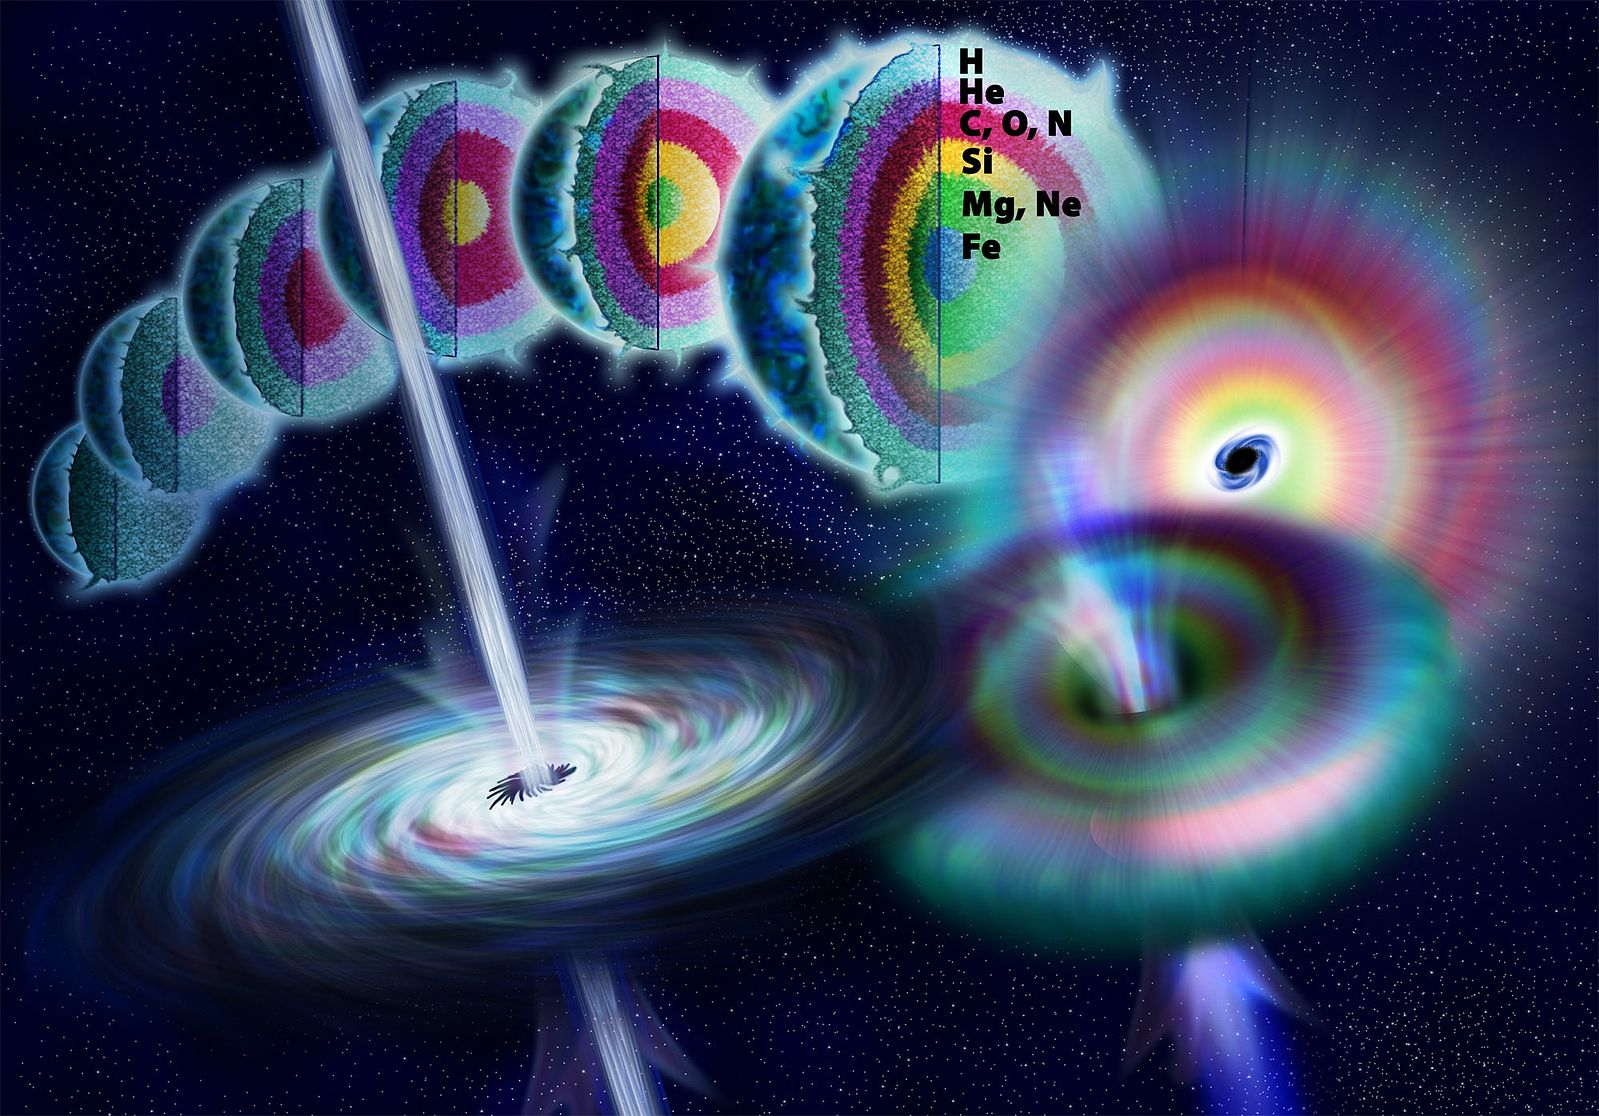
\includegraphics[width=130.0mm]{images/Gamma_ray_burst.jpg}
\caption{The life cycle of a massive star. When fusion stops the collapsing star releases energy in the form of jets observed as a gamma-ray burst}
\end{figure}

One of the most accepted theories describe GRBs as collisions of highly relativistic outflow of the accelerated jets \cite{grb10}. For most of the observed GRBs the prompt $\gamma$-ray emission was followed by a longer-lasting afterglow in soft X-ray, optical or radio waves \cite{grb11}. This is due to the propagation of a relativistic shockwave through the medium that surrounds the burst. Observations proved that GRBs are at cosmological distances \cite{grb12}. The farthest GRB observed was at a distance of z=9.4. The avarge short GRBs lie at a distance of z=0.5. The long GRBs are even farther away, on avarage at z=2. The energy that is released in such an event is tremendous, about 10 erg. Long GRBs have been linked to the brightest regions of galaxies those that contain the most massive stars \cite{grb14}. %The relativistic outflow of LGRBs has a bulk Lorentz factor of $\Gamma\sim$300 [5]. The afterglow observations indicate that a geometrical beaming of the LGRBs radiation has an opening angle of $\sim$5 \cite{grb15}.

\begin{figure}[H]
\centering
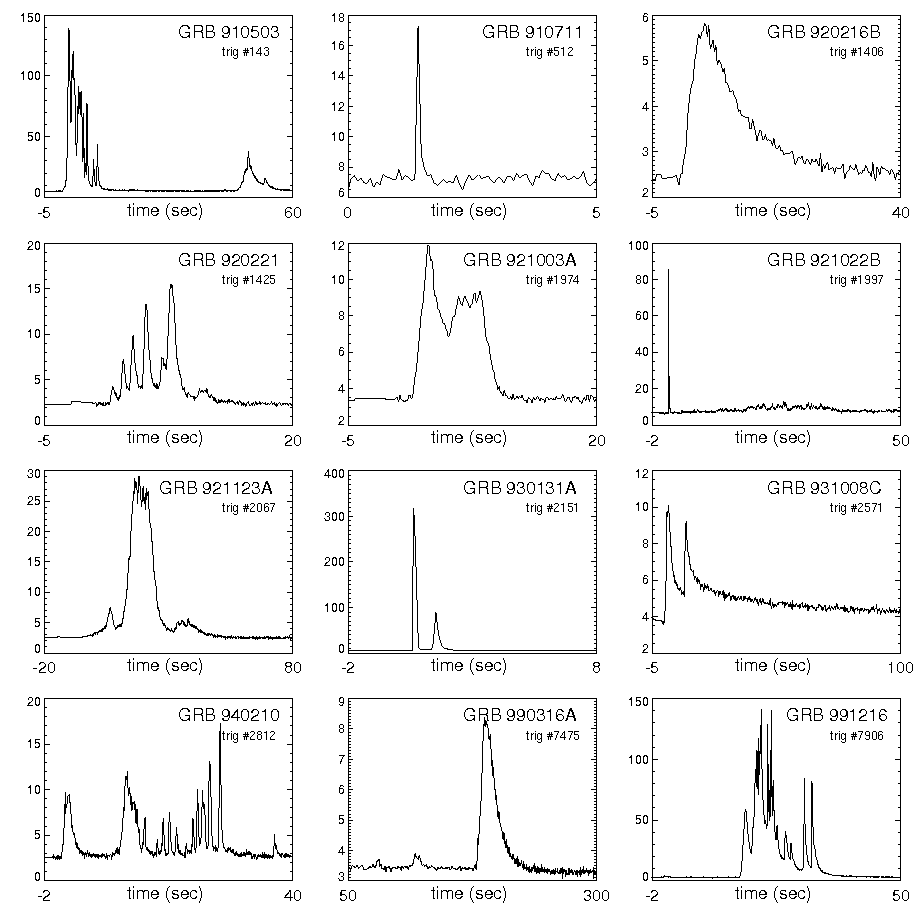
\includegraphics[width=130.0mm]{images/GRB_BATSE_12lightcurves.png}
\caption{The light curves of 12 gamma-ray bursts observed by BATSE. The diversity of the curves is extraordinary. Events with a length from millisecond to tens of seconds exist either with smooth or highly variable light curves.}
\end{figure}

On the contrary, short GRBs are thought to originate in old populations. The theory that they originate from the merging of two neutron stars has been recently confirmed by detecting the gravitational waves from such an event. GW170818 was detected by the LIGO/Virgo collaboration in 2017 \cite{gravwave}. The electromagnetic counterpart of this gravitational wave event was detected as a short GRB by the Fermi/Gamma-ray Burst Monitor (GBM) and INTEGRAL instruments followed by the observation of the GRB’s afterglow and its host galaxy \cite{grb17}. Kilonovae producing infrared electromagnetic radiation due to the radioactive decay of heavy r-process nuclei that are produced and ejected almost isotropically during the merger process \cite{grb18}.

\begin{figure}[H]
\centering
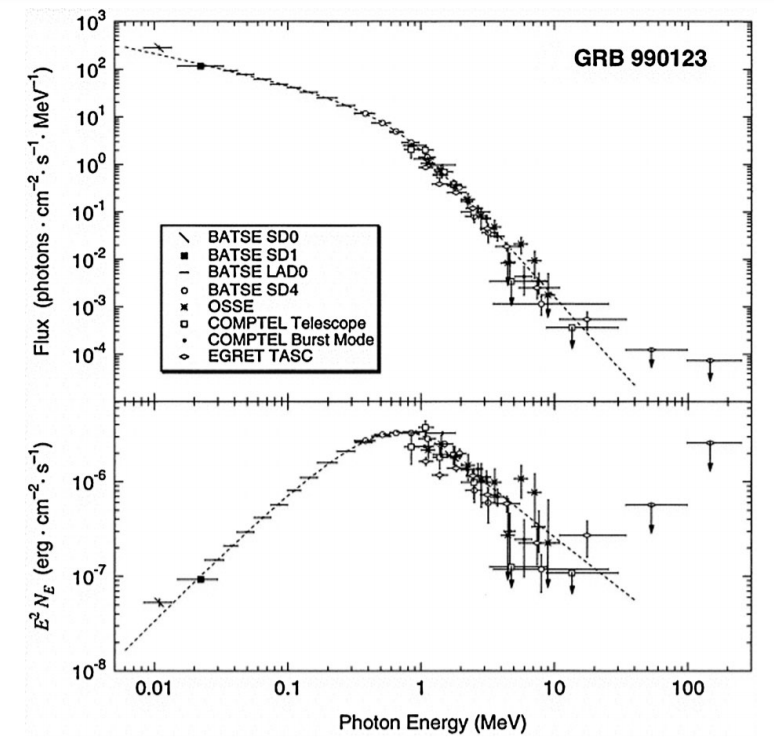
\includegraphics[width=130.0mm]{images/grb_spectra.png}
\caption{The band function of GRB 990123 $\cite{grb_spectra}$}
\label{fig:grb_band}
\end{figure}

\subsection{Open questions on gamma-ray bursts}

Despite the fact that GRBs have been studied for more than fourty years many questions are still not understood about their physics\cite{grb19}. In the following the main open questions are listed:

\begin{itemize}
\item{Classification: some of the observed light curves can not be classified into short and long GRBs, such as the ultra-long GRBs.}
\item{Central engine: in most cases it is thought that a black hole is formed after the merging of neutron stars and core collapse of massive stars. Although there are models that predict the birth of a magnetar. The most exotic theories predict the birth of a quark star that has never yet been observed.}
\item{Acceleration mechanism of the jets: How particles are accelerated to a velocity of a Lorentz-factor of 300 in the shock waves is not yet understood.}
\item{GRB jet composition: there are two possible driving forces behind the acceleration of jet material. The first one is magnetic field dominated and the other one is dominated by baryons. As the acceleration of particles is not yet fully understood, it is not known whether protons can be accelerated to ultra-high energies or not. These could produce Ultra-High Energy Cosmic Rays.} 
\item{Radiation mechanism: there are several physical processes that create the $\gamma$-ray spectrum of GRBs, that is called  the "Band" function. The following three processes are though to be the main contributors to the spectrum: synchrotron radiation, synchrotron self-compton radiation and Compton up-scattering of thermal photons.}
\item{First stars: different population of stars on avarage have different masses. Models predict that population III stars end their life with a black hole that has a mass about ten times bigger than population I and II stars. The progenitors of GRBs can be classified into populations by their redshifts \cite{grb20}.}

\end{itemize}

\subsection{Search for the electromagnetic counterparts of gravitational wave events}

Multi-messenger astronomy is based on the investigation of astronomical objects with disparate "messengers". It opened a possibility gather information in different ways to understand astrophysical objects. Until 2017 the three messenger were electromagnetic radiation, cosmic rays and neutrinos. 2017 opened a new era in multi-messenger astronomy as the electromagnetic counterpart of GW signal GW170817 was detected by the LIGO/Virgo collaboration. The source of this signal was the short GRB 170817A \cite{grb21}, a binary neutron star merger \cite{grb17}. 

This historical detection occured on August 17, 2017. The Fermi satellite detected the (short) GRB 170817A, approximately 1.7 s after the LIGO-Virgo detector network observed a GW signal GW170817. The origin of this source was a neutron-neutron star merger. The source was localized  in a sky region of 28 deg$^{2}$ (with 90 \% confidence). 

After the detection of the GRB signal, several space and earth based observatories in a wide range of wavelengths started the investigation of the source. The discovery of a bright optical transient linked to the GRB was discovered in NGC 4993. Observatories involved in the investigation included Chandra X-ray Observatory \cite{grb23}, INTEGRAL \cite{grb22}, Swift and Nuclear Spectroscopic Telescope ARray (NuSTAR). A blue kilonova associated with this event was detected \cite{grb24}. It is important to emphasize that not only neutron-neutron star mergers but neutron star-black hole and black hole-black hole mergers can emit electromagnetic signal \cite{grb25}. Therefore all short GRBs can be investigated with multi-messenger astronomy in the future. As LIGO is constantly upgrading its detectors, gravitational waves will be detected more often. An even more sensitive gravitational wave detector is under construction, callled Kamioka Gravitational Wave Detector (KAGRA). First scientific measurements will be taken in the 2020s \cite{grb26} with this device.

\subsection{Gamma- and X-ray detectors in space}

Almost all types of detectors starting from semiconductor based detectors to gas-filled detectors have been used in space. In the case of search for GRBs the detection of x-rays is the most relevant. Several types of detectors can be used for detecting $\gamma$ photons\cite{grb30}, for example the semiconductor based  German Position Sensitive Proportional Counters (PSPC) of the ROSAT X-ray telescope. For our satellite the size of the detector is limited, therefore the best option was to choose scintillators. Mostly used scintillators in space include inorganic crystal scintillators, for example NaI(Tl) or CsI(Tl), and plastic scintillators. CsI(Tl) was chosen as the detector of the Camelot CubeSat due to its high light yield.

\subsection{Current missions observing gamma-ray bursts}

This subsection provides an overview of the existing missions that are aimed to detect GRBs. Field of view (FOV) and localization accuracy are chosen to compare them with the CAMELOT mission. The proposed design of the CAMELOT satellites has the advantage of a large field of view and a high localization accuray. The main idea is that each CubeSat will detect GRBs at the same time. By measuring the time difference between the triggering of each satellite, the GRB soure can be localized by triangulation. By using more than nine satellites, the constellation achieves all sky coverage and localization accuracy.

The planed localization accuracy might reach $\sim$10'. While providing a good localization accuracy, the field of view would be even larger than  that of the INTEGRAL/SPI-ACS and Fermi.

The size and mass of the Camelot CubeSat is less than 1\% of the Fermi telescope. Therefore from a fraction of the cost several satellites could be built and deployed in orbit. Having several satellites also provides redundance.

\begin{figure}[H]
\centering
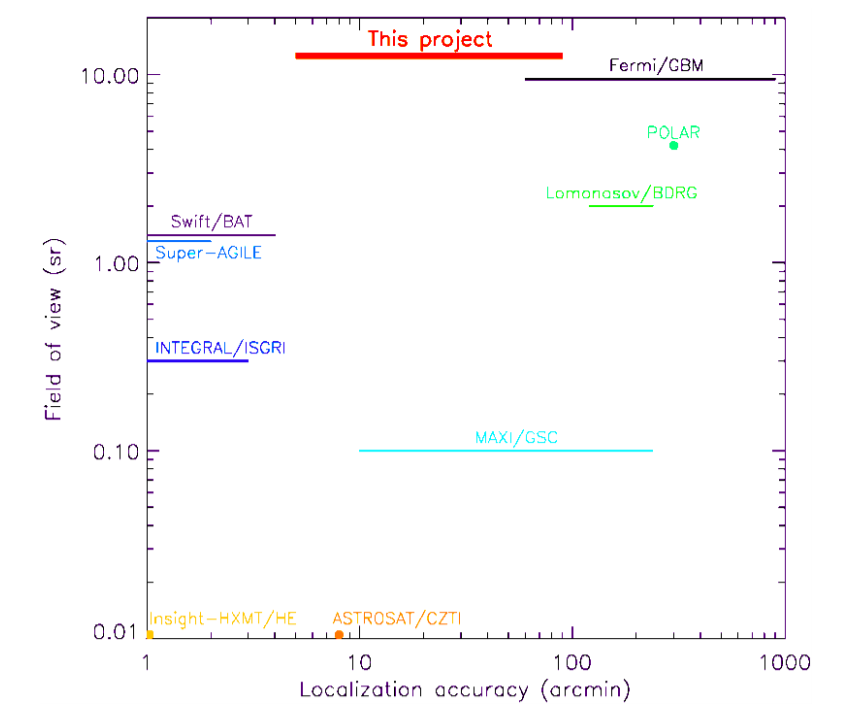
\includegraphics[width=130.0mm]{images/fovvsloc.png}
\caption{The field of view and localization accuracy of several missions including the CAMELOT CubeSat.}
\end{figure}

The following list includes the most relevant, currently ongoing missions looking for GRBs:

\begin{itemize}
\item Fermi \cite{grb28} was launched in 2008 and its main instruments are the Gamma-ray Burst Monitor and the Large Area Telescope (LAT). 
\item Neil Gehrels Swift Observatory (Swift) \cite{grb31} was launched in 2005 with its main instruments, those are the Burst Alert Telescope (BAT),  the X-ray Telescope (XRT), and the UV/Optical Telescope (UVOT).
\item INTErnational Gamma-Ray Astrophysics Laboratory (INTEGRAL) \cite{grb32} was launched in 2002. The most succesfull instruments on board include are the Anti-Coincidence Shield of the SPectrometer of INTEGRAL (SPI-ACS) and the Integral Soft Gamma-Ray Imager (ISGRI) detector layer of the "Imager on Board the Integral Satellite (IBIS)" detector.
\item Astro-Rivelatore Gamma a Immagini Leggero (AGILE)  \cite{grb34} was launched in 2007 and its Hard X-ray Imaging Detector (Super-AGILE) detected several GRBs.
\item CALorimetric Electron Telescope (CALET)  \cite{grb35} / Gamma-Ray Burst Monitor (CGBM), was launched in 2015 and it is placed on the International Space Station (ISS).
\item Monitor of All-sky X-ray Image (MAXI) \cite{grb36}, started nominal observation in 2009. Its instrument Gas Slit Camera (GSC) detects GRBs. This instrument is placed on ISS.
\item Gamma-ray Burst Polarimeter POLAR 14 \cite{grb37}, was launched in 2016 and is dedicated to the measurement of $\gamma$-rayGRB polarization.
\item Lomonosov/BDRG \cite{grb38}, was launched in 2016. The BDRG instrument on board detected several GRBs.
\item The Hard X-ray Modulation Telescope (Insight-HXMT) \cite{grb39} was launched in 2017. It has the high energy X-ray telescope (HE), the medium energy X-ray telescope, and the low energy X-ray telescope.
\item ASTROSAT \cite{grb40} was launched in 2015 and its Cadmium Zinc Telluride Imager (CZTI) has already detected many GRBs.
\item Reuven Ramaty High Energy Solar Spectroscopic Imager (RHESSI) \cite{grb41}, was launched in 2002. It is designed to study hard x-ray and gamma-ray emission from solar flares, however it is also efficient instrument to detect non-solar gamma-ray events like GRBs.
\end{itemize}


%\subsection{Currently operating GRB collection and alert networks}

%Our project can potentially contribute to some of the currently operating GRB collection and alertnetworks such as the following ones:
%The InterPlanetary Network (IPN) 27 \cite{grb42} which derives the positions of fast gamma-ray transients of all kinds by triangulation. Numerous spacecraft and instruments participate in the network at the Earth’s orbit as well as in the interplanetary space. It detects about 350/year.
%The Gamma-ray Coordinates Network (Transient Astronomy Network) (GCN/TAN) 28 provides information about GRBs in real-time to the world community. The network provides the real-time (and near real-time) distribution of GRB locations, images, spectra, and lightcurves detected by various spacecraft and the distribution of follow-up observation reports.
%The Global Relay of Observatories Watching Transients Happen (GROWTH) 29 is an international scientific collaborative project studying the astronomical transients.

%\subsection{Current GRB Follow-up observations}

%This cubesat project will provide high precision localization accuracy of GRBs allowing efficient follow-up observations by existing ground based observatories. There are several observatories world-wide to perform photometric or spectroscopic observations of GRB afterglows, for example:
%The Mobile Astronomical System of TElescope Robots (MASTER) 30 \cite{grb43} is a global network of robotic telescopes for very fast positioning and follow up of GRBs.
%The Burst Optical Observer and Transient Exploring System (BOOTES) network of robotic telescopes for follow up observations of GRBs. 31 \cite{grb44} is a world wide The Robotic Optical Transient Search Experiment (ROTSE) 32 [101] are telescopes which operate at sites around the world and follow GRBs.
%Pi of the Sky 33 [102] is a system of detectors designed for continuous observation of night sky looking for optical flashes of astrophysical origin, in particular for GRBs.
%Several other telescopes and observatories which provide measurements in optical, infra-red or radio bands are also, e.g.: Gamma-Ray Burst Optical/Near-Infrared Detector (GROND) 34 , the Palomar 60 inch telescope 35 , Rapid Eye Mount (REM) 36 , Livermore Optical Transient Imaging System (Super- LOTIS) 37 , Télescopes à Action Rapide pour les Objets Transitoires (TAROT) 38 , Gran Telescopio Canarias (GTC) 39 , ESO Very Large Telescope (VLT) 40 , Nordic Optical Telescope (NOT) 41 , Observatorio Astronómico Nacional on the Sierra de San Pedro Mártir 42 , Cerro Tololo Inter-American Observatory (CTIO) 43 , Telescopio Nazionale Galileo (TNG) 44 , Gao-Mei-Gu (GMG) station of Yunnan Observatories 45 , Observatorio de Sierra Nevada (OSN) 46 , United Kingdom Infrared Telescope (UKIRT) 47 , Very Large Array (VLA) 48 , Atacama Large Millimeter/Submillimeter Array (ALMA) 49 , James Clerk Maxwell Telescope 50 , Arcminute Microkelvin Imager which robotically triggers on Swift GRBs (AMI-GRB) 51 .

\subsection{The CAMELOT satellite}

The CAMELOT satellite platform is being developed by C3S LLC, in Budapest. There would most likely be four scintillators on the CAMELOT satellite, on two neighbouring sides of the satellite, two scintillators each. The scintillators will have a case either from aluminium or carbon fibre.

\begin{figure}[H]
\centering
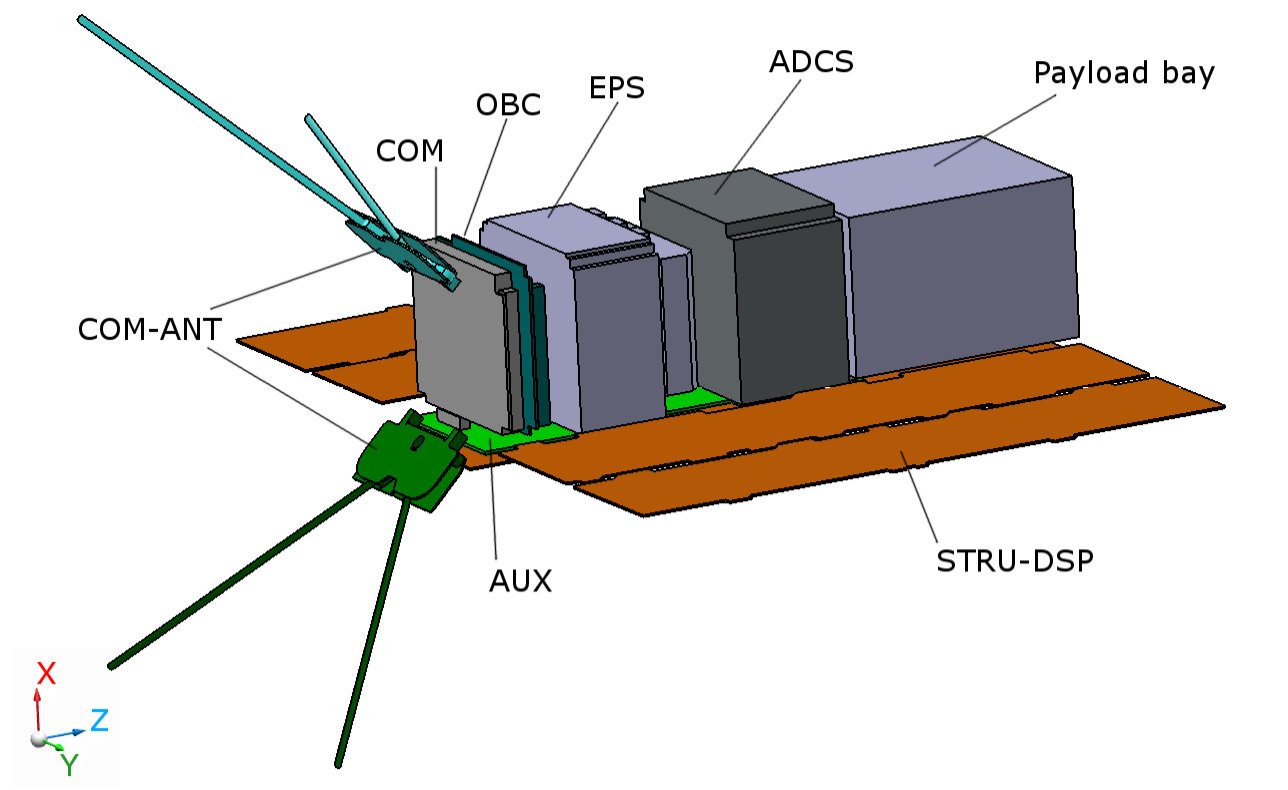
\includegraphics[width=130.0mm]{images/satellite_modules.png}
\caption{The modules of the satellite (Courtesy of C3S LLC) \cite{drawing}}
\end{figure}

The CAMELOT satellite will consist of the following modules:

\begin{itemize}
\item On-Board Computer [OBC] is responsible for the control of all the satellite’s sub-systems. OBC performs housekeeping and collects payload data and archives it in its internal storage.
\item Electrical Power System [EPS] is responsible for managing primary and secondary power sources and distributing power at appropriate voltage levels to on-board subsystems.
\item COM UHF Transceiver [COM] provides an RF communication link between the Ground Segment and the satellite. The COM codes are received messages from the OBC and are transmitted to the Ground Segment. Furthermore, the COM decodes the received RF messages from the Ground Segment and transmits them to the OBC.
\item Attitude Determination and Control System [ADCS] determines and controls the altitude of the satellite.
\item Auxiliary Electronics [AUX] subsystems control the deploying mechanisms and monitor the solar arrays. The Aux subsystem also contains the rigid backplane of the satellite; therefore, it also connects the subsystems.
\item Structure [STRU]
\item Ground Support Equipment [EGSE]
\end{itemize}

\subsection{The detection of GRBs}

In the case of our satellite, the detection of $\gamma$ photons from GRBs will be carried out by a Caesium Iodide scintillator doped with Tellurium. This is the most popular alkali halide scintillation crystal apart from NaI(Tl). The $\gamma$ photons create scintillation, thus thousands of optical photons in the scintillator. These photons will be detected by Silicon Photomultiplier device called Multi Pixel Photon Counter, MPPC for short. This is by far the best and most compact solution as the size of cubesat standard is limited to be $\sim$300x75x5 mm$^{3}$. The first tests were carried out by a single MPPC readout, which was followed by a design with two MPPCs to maximize the light yield and minimalize the noise. The size of the Hamamatsu MPPC is 6x6 mm$^{2}$. The scintillators will be placed onto the surface of the satellite as can be seen in fig. \ref{fig:scints}. While fig. \ref{fig:schem} shows the experimental setup used for the tests.

\begin{figure}[H]
\centering
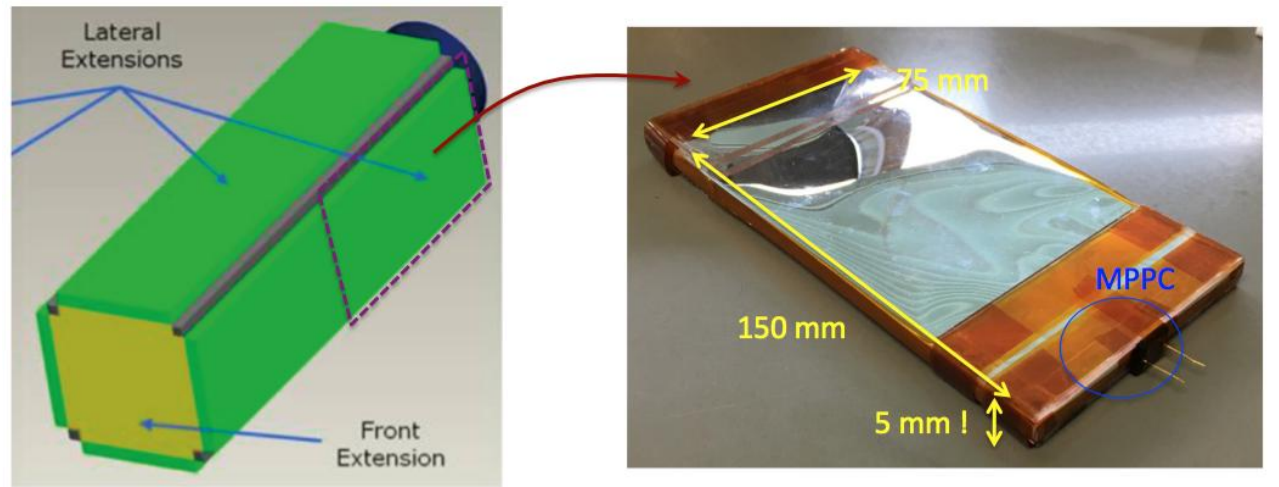
\includegraphics[width=130.0mm]{images/scint_on_sate.png}
\caption{Side extensions including the CAMELOT satellite (left, based on QB50 system requirements and recommendations) where scintillators are placed and a wrapped scintillator with the MPPC read out (right) \cite{kento}}
\label{fig:scints}
\end{figure}

The large area and small thickness of the scintillator makes it challenging for the read out as optical photons have to be reflected several times to reach the MPPC. Two factors play a role here, the self absorption of the reflectivity of the tape that is used to cover the scintillator. The length of the self absorption is in the order of a meter and the reflectivity of the ESR tape, which is above 99 \% can be seen in fig. \ref{fig:refl}. The idea that we came up is using two MPPC-s with coincidence. This results in a smaller leakage current (noise) as the noise has a poissonian statistic. Therefore the noise is "random" and a trigger from both of the MPPC is unlikely. The other advantage is the increased photon yield due to the double of the photon collection area. The difference between one and two channel readout can be seen in fig. \ref{fig:spectras_meas}.

\begin{figure}[H]
\centering
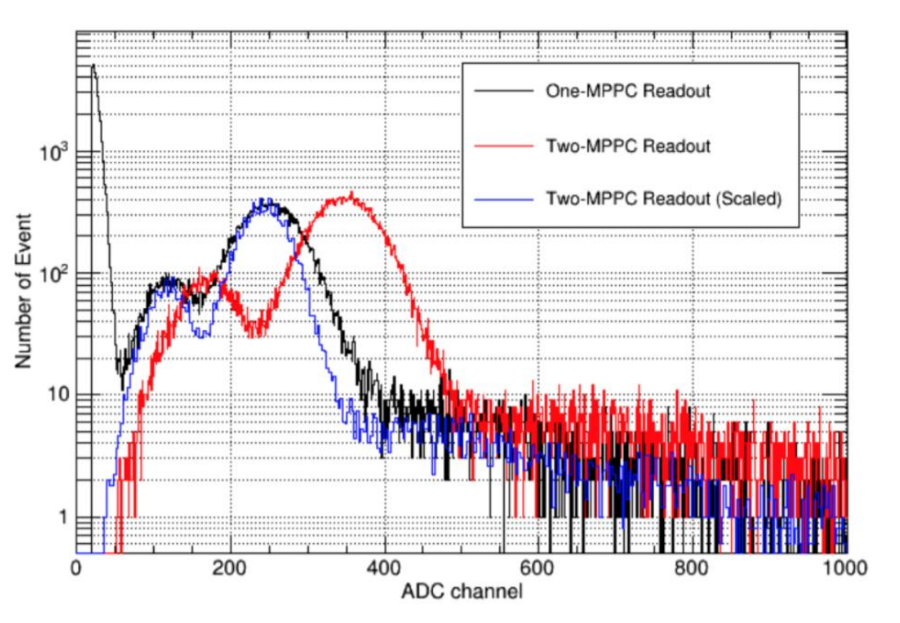
\includegraphics[width=130.0mm]{images/histo_for_det.png}
\caption{Energy spectra obtained by collecting the signal of 1 million $\gamma$ with the one channel and the two channel read out \cite{kento}}
\label{fig:spectras_meas}
\end{figure}

\subsection{The Geant4 platform}

The most used software in particle physics are MCNPX, FLUKA and Geant4. For this thesis Geant4 was chosen as it is the best for simulation of several types of particles at the same time and building up the geometry of detectors is propably the most convinient in this software. 

Geant4 \cite{geant1, geant2, geant3} (for GEometry ANd Tracking) is a platform for "the simulation of the passage of particles through matter," using the Monte Carlo method. It has been developed at CERN for more than three decades by dozens of physicst and programmers. The cross sections for all interactions between matter and particles are included in this software. It is an object orianted programming platform in C++. Its development, maintenance and user support are taken care of by the international Geant4 Collaboration. Areas in science that have used Geant4 vary widely from the design of complex medical machines to accelerator, nuclear physics, high energy physics and space applications. Several thousands of people use it all around the world.

\begin{figure}[H]
\centering
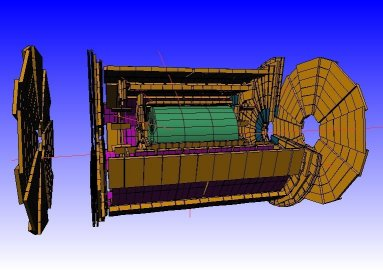
\includegraphics[width=130.0mm]{images/AtlasHalf.jpg}
\caption{The Geant4 simulation of the whole ATLAS experiment}
\end{figure}

The Geant4 platform includes all the important features required in the full simulation of an experiment from handling the geometry of the detector and readout, tracking of particles in the detectors for visualization.

\pagebreak

\subsection{The experimental setup}

In order to understand and charaterize the behaviour of the large-area CsI(Tl) scintillator detector and the MPPC readout; an experimental setup was built in Hiroshima, Japan. The experimental setup provided vital information for the simulation, mostly for the position dependence of the light yield. Different $\gamma$ sources were used, mostly an $^{241}$Am source. 

\begin{figure}[htbp]
 \centering % \begin{center}/\end{center} takes some additional vertical space
 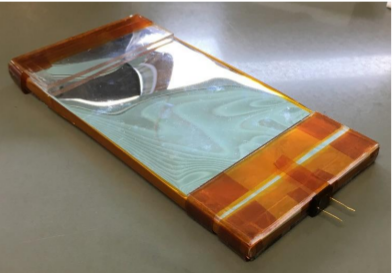
\includegraphics[width=.4\textwidth,origin=c,angle=0]{images/1channelsetup.png}
 \qquad
 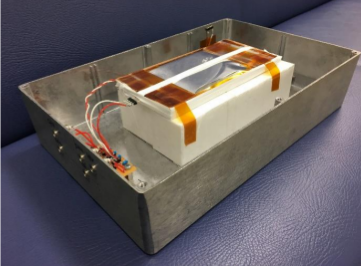
\includegraphics[width=.4\textwidth,origin=c,angle=0]{images/1channelsetupbox.png} 
 % "\includegraphics" from the "graphicx" permits to crop (trim+clip)
 % and rotate (angle) and image (and much more)
 \caption{\label{fig:i} The scintillator on the left and the cage holding the setup on the right \cite{kento}}
 \label{fig:schem}
 \end{figure}

The detector was wrapped in a so called ESR foil that is designed to reflect as much light as possible. In fig. \ref{fig:refl} the reflectivity of this tape can be seen depending on the wavelength of the photons, exceeding 99 \% for most of the relevant spectrum. It is important as the optical photons have to be reflected several times in order to be read out with the small effective are of the MPPC. This reflectivity was included in the simulation.


\begin{figure}[H]
\centering
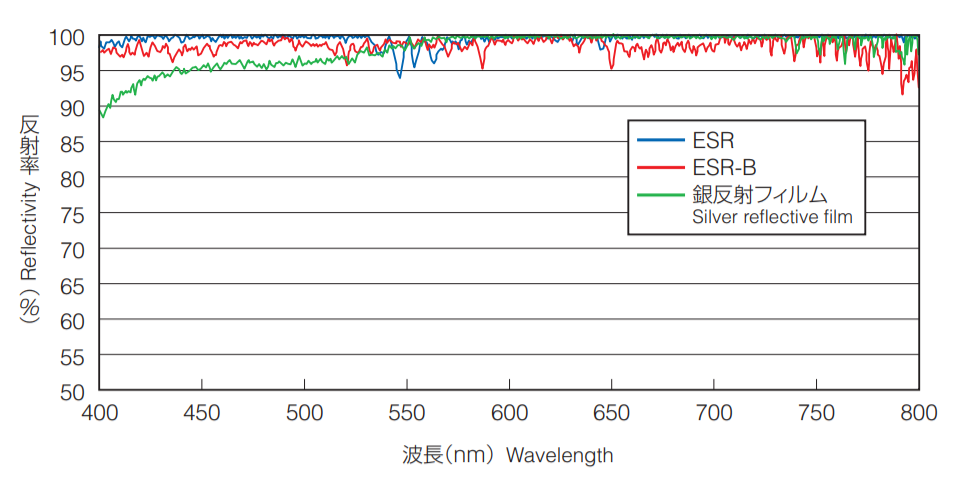
\includegraphics[width=130.0mm]{images/reflectivity.png}
\caption{The reflectivity $\cite{scinti}$ of the ESR tape that was used to wrap the scintillator in order to increase the light yield. This data was included in the simulation.}
\label{fig:refl}
\end{figure}

The CsI(Tl) scintillator used is produced by AmCrys \cite{scinti}. The dimensions of this detector are 150 mm x 75 mm x 5 mm, the largest possible size that can fit onto the surface of the satellite. The spectra of the optical photons produced in the scintillation process can be seen in fig. \ref{fig:scint_yield}. An aluminium case of 2mm is used, the same as planned for the mission in space. The time constant for the scintillation of the detector was 200 ns.

\begin{table}[h!]
\begin{center}
\begin{tabular}{ |c|c|c|c|c|c|c|c|c|} 
 \hline
 Energy [eV] & 3.54 & 3.10 & 2.76 & 2.48 & 2.36 & 2.25 & 2.07 & 1.91\\\hline
 Relative emittance & 0.02 & 0.1 & 0.3 & 0.6 & 0.9 & 1.0 & 0.7 & 0.4 \\\hline
 Refractive index & 1.59 & 1.57 & 1.54 & 1.54 & 1.54 & 1.54 & 1.54 & 1.54 \\\hline
 Absorption lengh [cm] & 50 & 50 & 50 & 50 & 50 & 50 & 50 & 50  \\\hline
\end{tabular}
\end{center}
\caption{The parameters of the CsI(Tl) scintillator used in our experiment}
\end{table}


\begin{figure}[H]
\centering
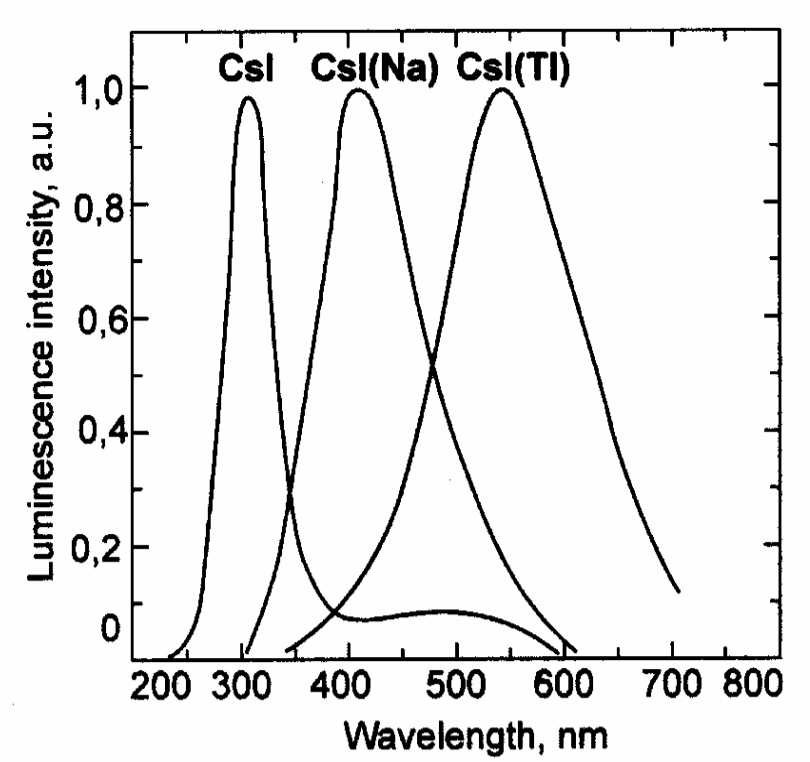
\includegraphics[width=130.0mm]{images/spectracsitl.png}
\caption{The emitted scintillation light spectra of three types of scintillators. In our experiment CsI(Tl) was used}
\label{fig:scint_yield}
\end{figure}

The MPPC chosen for this satellite is one of the latest models (HAMAMATSU S13360-6050CS) \cite{qe}. It has an effective area of 6mm x 6mm. The photon detection efficiency of this specific model can be seen in fig. \ref{fig:qe}.

\begin{figure}[H]
\centering
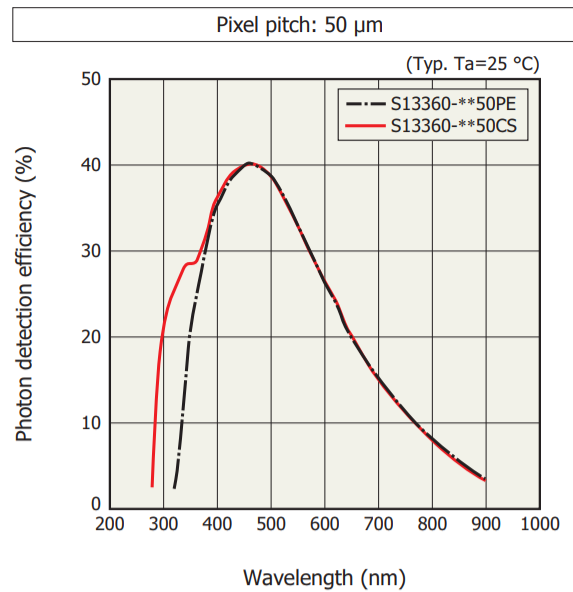
\includegraphics[width=130.0mm]{images/qe.png}
\caption{The photon detection efficiency $\cite{qe}$ of the MPPCs used for the readout of the scintillators. This data was included in the simulation.}
\label{fig:qe}
\end{figure}

\pagebreak

\subsection{The readout of the detector}

The response of the MPPC detector used depends on temperature. Therefore the experimental setup was placed in a thermally controlled chamber (ESPEC LU-113) keeping the temperature at 25$^{\circ}$. Two setups were investigated. The first one with a single MPPC readout placed in the middle of one side of the scintillator. In the other case two MPPCs were utilized symmetrically placed on one side of the detector.

For the single MPPC readout setup a commercial charge-sensitive preamplifier (CLEAR-PULSE 5028), a shaping amplifier (EG\&G ORTEC 571), and an ADC (AMPTEC MCA800A) were used to obtain an electric signal read out by a PC. The shaping time was set to 1 $\mu$s.

\begin{figure}[h!]
\begin{center}
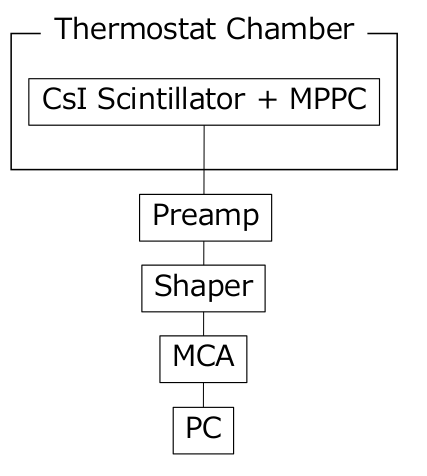
\includegraphics[width=80.0mm]{images/1channelelectronics.png}
\caption{The schematic design of the readout of the MPPC for the 1 channel configuration \cite{kento}}
\label{fig:el1ch}
\end{center}
\end{figure}

For the case of the two-channel read out an FADC board was utilized that contains all the necesarry electronics to read out the signal of the MPPC with an additional coincidence unit. This board was developed for the astrophysical polarimetry mission PoGO+. The shaping time was set to 2.2 $\mu$s in this case. The breakdown voltages of the two-MPPCs are almost the same–50.82 and 50.87 V–at 25 C. We used a KEITHLEY 2400 to supply the operational voltage of 53.4 V.

\begin{figure}[h!]
\centering
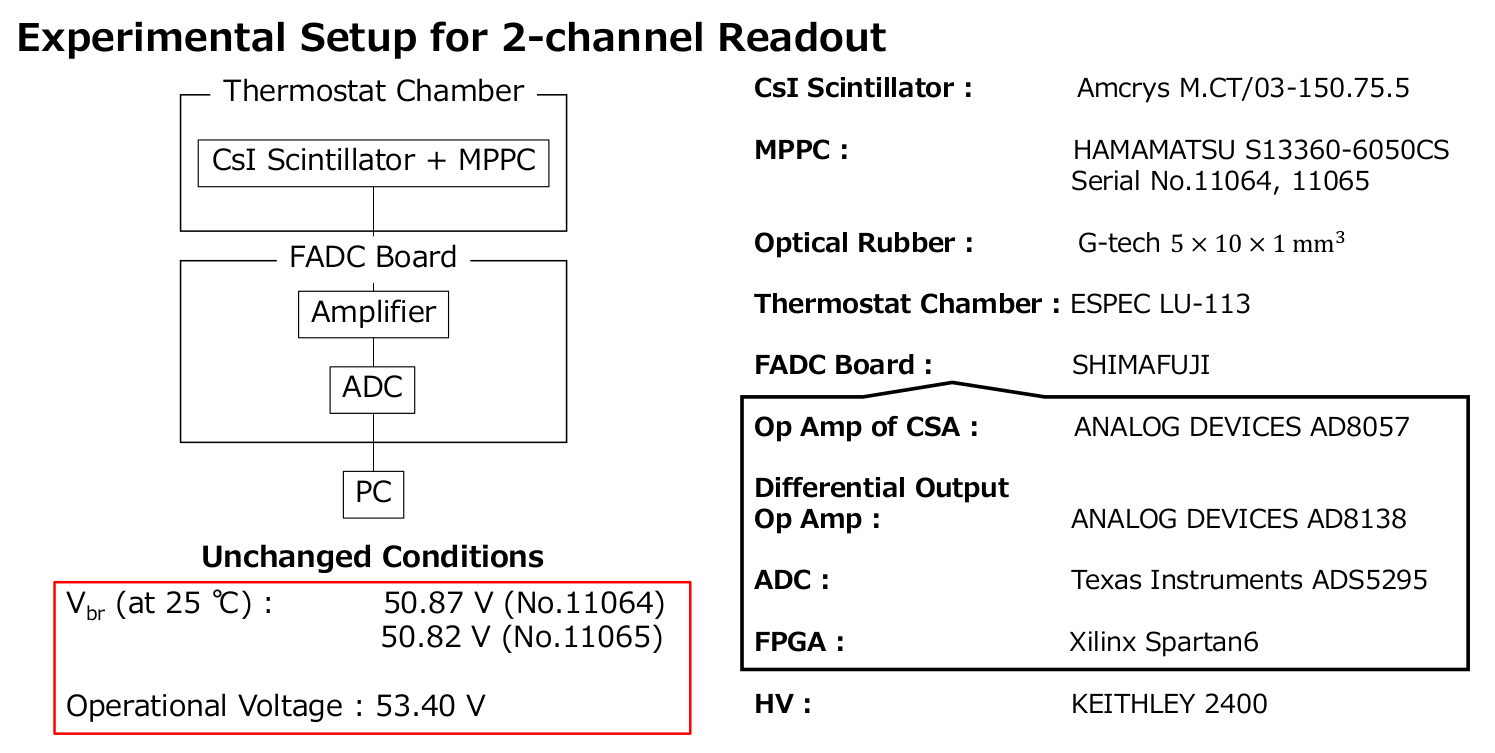
\includegraphics[width=80.0mm]{images/2channelelectronics.png}
\caption{The schematic design of the readout electronics of the 2 channel setup \cite{kento}}
\end{figure}

%  CsI_mt->AddConstProperty("RESOLUTIONSCALE",1.0);
%  CsI_mt->AddConstProperty("SLOWTIMECONSTANT",200.*ns);
%  CsI_mt->AddConstProperty("YIELDRATIO",1.0);
  
% G4double glass_RIND[lxenum]={1.49,1.49,1.49};
%  G4double glass_AbsLength[lxenum]={420.*cm,420.*cm,420.*cm};  
%  G4double reflectivity[num] = {0.995, 0.995};
%G4double photocath_EFF[num]={1.,1.}; //Enables 'detection' of photons
%  G4double photocath_ReR[num]={1.92,1.92};
%  G4double photocath_ImR[num]={1.69,1.69};

\pagebreak

\subsection{1 channel setup}

The $\gamma$ source that was used to test the experimental setup was choosen to be an $^{241}Am$. The reason for this is that the peak of the energy spectrum of the $\gamma$ photons from GRBs is at 50 keV which is very close to the peak of the $^{241}Am$ that is 59.5 keV. The activity of the source at the time of the experiment was 471 kBq. The source was collimated to a beam that hit the surface of the scintillator on a circle with a radius of 10 mm. The distance of the source from the scintillator was 13.5 mm. 

\begin{figure}[h!]
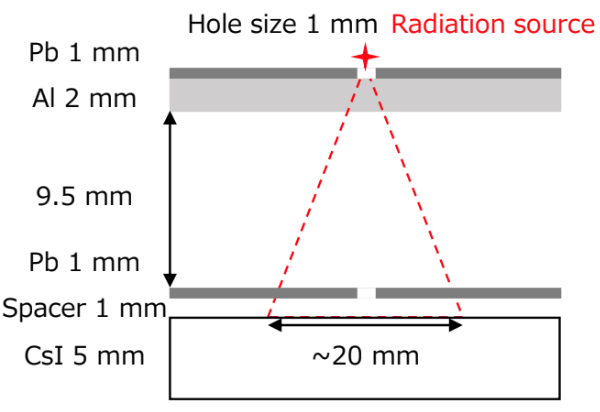
\includegraphics[width=150.0mm]{images/irradiation.png}
\caption{The $^{241}$Am $gamma$ source was placed in a collimator system as can be seen on the image \cite{kento}}
\label{fig:this_set}
\end{figure}

Therefore the solid angle of the part of the whole sphere where $\gamma$s could be detected was 
$$\Theta = 2 \pi (1-cos(\theta)) = 1.234 sr$$

\pagebreak

\subsection{2 channel read out setup}

In order to maximize the light yield, thus the signal of the detector and minimize the noise with coincidence a 2 channel setup was tested.  In fig. \ref{fig:schem2c} this setup can be seen with the MPPCs placed symmetrically onto the scintillator.

\begin{figure}[h!]
\centering
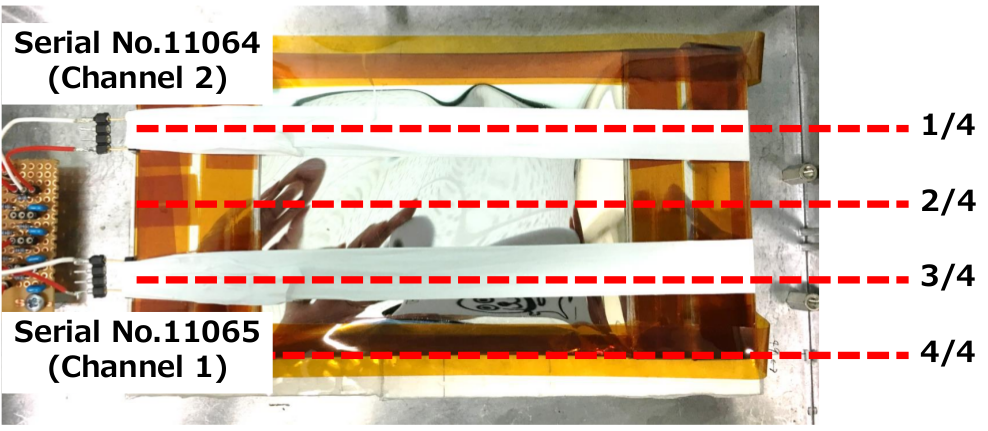
\includegraphics[width=130.0mm]{images/2channelsetup.png}
\caption{The MPPCs for the 2 channel readout are positioned symmetrically from the center of the scintillator \cite{kento}}
\label{fig:schem2c}
\end{figure}

In order to simulate the satellite with the two channel read out setup, first this configuration was tested. The simulation of this setup can be seen in fig. \ref{fig:sim2ch}. The $\gamma$ source was collimated with a lead sheet that was drilled in 9 places. The optical photons that were detected are shown only in the simulation. The two read out volumes (red) correspond to the MPPCs.

\begin{figure}[h!]
\centering
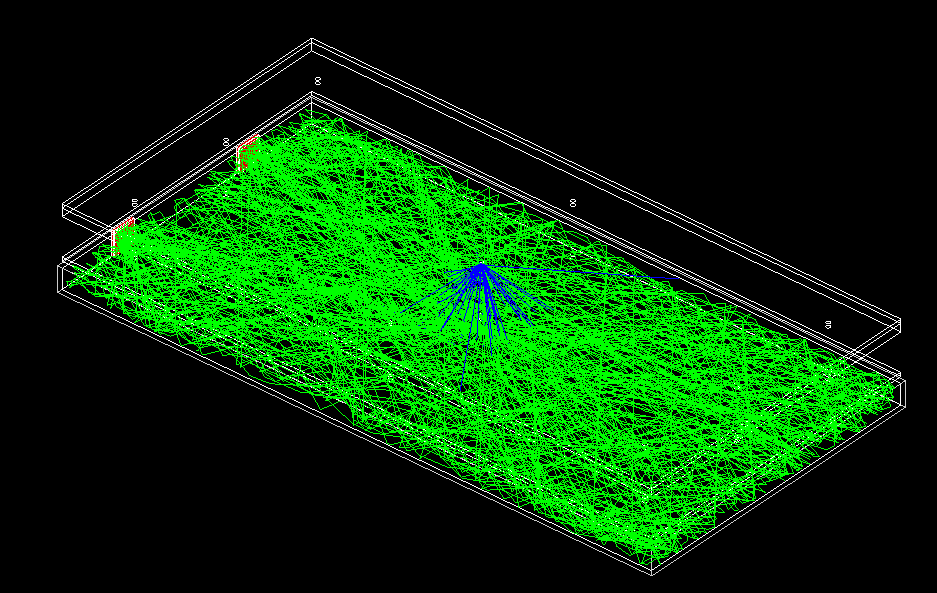
\includegraphics[width=130.0mm]{images/2channel.png}
\caption{Simulation of 100 $\gamma$s emitted from the source. The blue lines represent the track of the $\gamma$s and the green lines represent the track of the optical photons created by scintillation. Only the photons that were detected are drawn.}
\label{fig:sim2ch}
\end{figure}

\pagebreak

\subsection{The satellite}

The direction of GRBs is isotropic in the sky as they are extragalactic objects. As the position of the scintillators is not decided yet it is important to understand which configuration would be the best in order to detect as many GRBs as possible. Therefore it is vital to understand how the material of the satellite itself absorbs and scatters $\gamma$-rays. The satellite consists of several modules with specific shapes and material contents. Therefore building up the whole geometry and material composition was not possible in Geant4, thus the model of the satellite had to be  imported into Geant4.

\begin{figure}[h!]
 \centering % \begin{center}/\end{center} takes some additional vertical space
 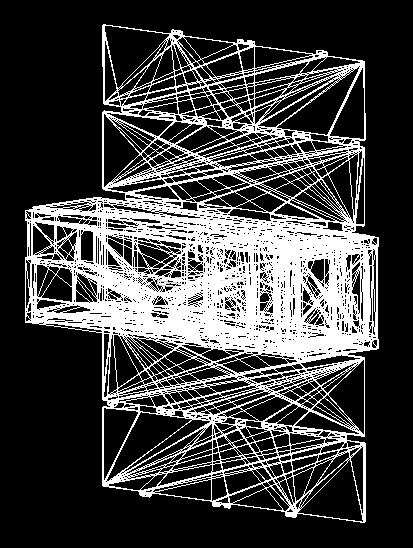
\includegraphics[width=.35\textwidth,origin=c,angle=0]{images/satellite.png}
 \qquad
 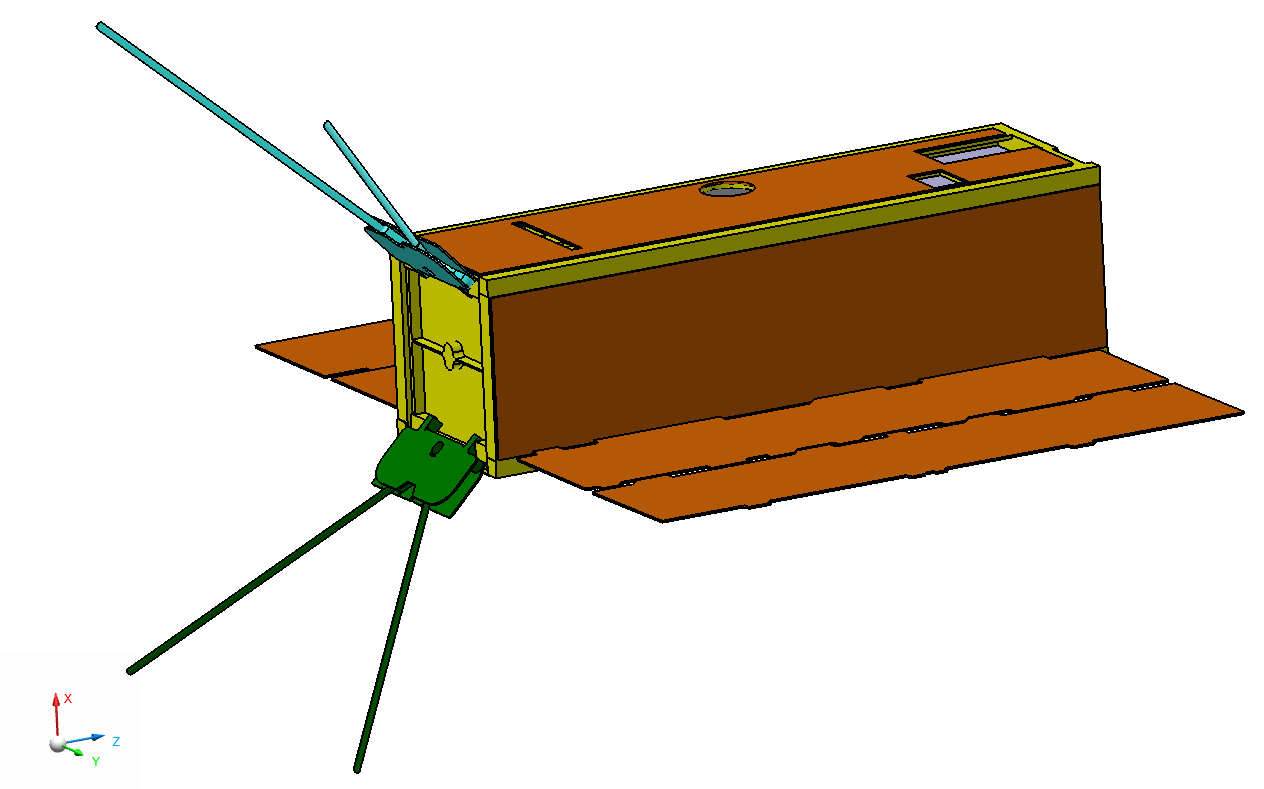
\includegraphics[width=.5\textwidth,origin=c,angle=90]{images/cad_sat.png} 
 % "\includegraphics" from the "graphicx" permits to crop (trim+clip)
 % and rotate (angle) and image (and much more)
 \caption{\label{fig:i} The CAD model of the satellite \cite{drawing} (on the right, Courtesy of C3S LLC) and the view of the imported model in Geant (on the left)}
 \end{figure}

Importing predefined CAD models into GEANT4 is not always possible or requires intermediate file format conversion to Geometry Description Markup Language (GDML) using commercial or third party software. CADMesh \cite{cadmesh} is a direct CAD model import interface for GEANT4 leveraging ASSIMP \cite{assimp} for reading the CAD files. In this work the CAD model of the satellite was exported to STL files. These files were imported by the CADMesh software to Geant4. The tesselation was done by the TETGEN \cite{tetgen} software.

\begin{table}[h!]
\begin{center}
\begin{tabular}{ |c|c|c|c|} 
 \hline
 Name of module & mass [g] & Type of material & Mass ratio [\%]\\\hline
 ADCS &	710	& Aluminum 6061-T6 &	50\\
			& & Copper Electric	& 25 \\
			& &  Glass Borosilicate 	& 25\\\hline
COM	& 	90	& 	Stainless Steel 	& 2\\
			& 	& Brass Generic		& 25\\
			& 	& Aluminum 7075-T73		& 40\\
			& 	& FR4 Glass-Epoxy sheet	& 	33\\\hline
EPS	& 	750	& 	FR4 Glass-Epoxy sheet		& 25\\
			& 	& Aluminum 6061-T6		& 75\\\hline
OBC	&	50		& FR4 Glass-Epoxy sheet	& 	100\\\hline
STRU	& 	980		& Aluminum 6061-T6	& 	100\\\hline
SP	& 	570		& Solar Panel	& 	100\\\hline
Payload	& 	100	& 	Aluminum 7075-T73	& 	100\\
 \hline
\end{tabular}
\end{center}
\caption{The mass ratio of materials that are used for the satellite (Courtesy of C3S LLC) \cite{drawing}}
\label{table:materials}

\end{table}

\pagebreak

The material composition of the satellite can not be exported to Geant4 from CAD files directly. Therefore an avarage material composition was calculated for all the modules. In table $\ref{table:materials}$ the material compositions of the 7 modules are listed. These materials, mostly alloys, consist of several elements. The Geant4 cross section database is built up only for elements. Therefore these materials had to be broken down to elements.

\begin{table}[h!]
\begin{center}
\begin{tabular}{ |c|c|c|c|c|c|c|c|c|c|c|c|c|} 
 \hline
%Material name & El. 1	& El. 1 m.r. & El. 2 & El. 2 m.r. &El.3	& El. 3 m.r. &El. 4	& El. 4 m.r. &El.	5& El. 5 m.r. &El.	6& El. 6 m.r. \\\hline
Material name & &&&&&&&&&&& \\\hline
Aluminum 6061-T6 &	Al & 96.90 &	Mg &	1.20 &	Si &	0.80 &	Fe &	0.70 &	Cu &	0.40 & &\\\hline		
Aluminum 7075-T73 &	Al &	88.60 &	Zn &	6.10 &	Mg &	2.90 &	Cu &	2.00 &	Si &	0.40 & &\\\hline		
%Stainless Steel A2-70  AISI 304 (EN 1.4301) &	Fe &	66.50 &	Cr &	20.00 &	Ni &	10.50	Mn &	2.00 &	Si &	1.00 & &\\\hline		
Stainless Steel &	Fe &	66.50 &	Cr &	20.00 &	Ni &	10.50	&Mn &	2.00 &	Si &	1.00 & &\\\hline		
Copper Electric  &Cu &	100.00 & & & & & & & & & &	\\\hline			
Glass Borosilicate &	Si &	42.10 &	O &	54.80 &	B &	3.10 & & & & & &\\\hline			
FR4 Glass-Epoxy &	Si &	23.39 &	O &	36.02 &	C &	37.04 &	H &	3.55 & & & &\\\hline		
Brass Generic &	Cu &	85.00 &	Zn &	15.00 & & & & & & & &\\\hline						
Solar Panel &	Ge &	38.00 &	Si &	24.00 &	O &	20.00 &	C &	13.00 &	H &	4.00 &	B &	1.00\\\hline
\end{tabular}
\end{center}
\caption{The chemical composition of materials in mass fraction that are used for the satellite (Courtesy of C3S LLC) \cite{drawing}}
\end{table}

\pagebreak

In fig. \ref{fig:sat_rad} the simulation of the satellite and the two channel read out setup can be seen. 100 $\gamma$ particles were used to shoot the satellite with a beam parallel to the plane of the scintillator. A $\gamma$-ray can be seen scattered into the scintillator and being detected.

\begin{figure}[h!]
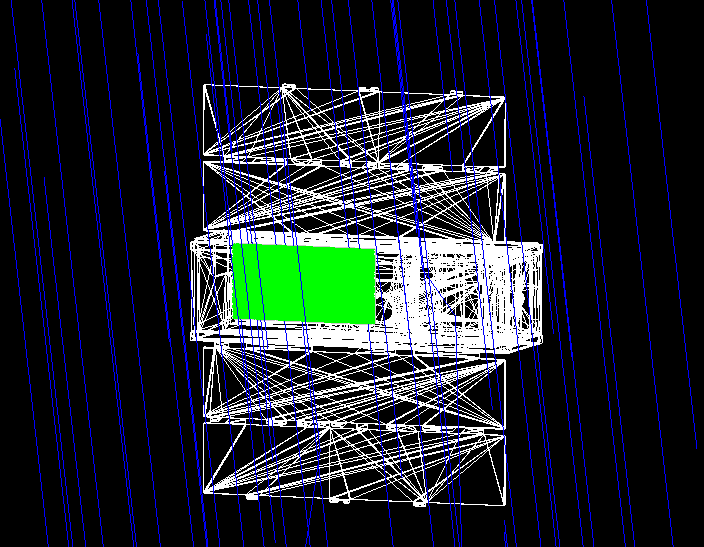
\includegraphics[width=150.0mm]{images/satellite_rad.png}
\caption{The satellite radiated by a parallel beam of 100 $\gamma$ particles. The scattered $\gamma$s induce signal in the detector.}
\end{figure}
\label{fig:sat_rad}

\pagebreak

\section{Results of the simulation}


\subsubsection{X-ray fluorescence}


The measured spectra of the scintillation light created by $\gamma$-rays (fig. \ref{fig:spectras_meas}) have a main peak that corresponds to the 60 keV $\gamma$s from the $^{241}$Am source. There is an additional peak with an amplitude of roughly 20 \% of the main peak. The physical process that is behind this is X-ray fluoresence. By default this process is not included in Geant4 simulations, thus I had to turn it on. A histogram with and without x-ray fluorescence can be seen in fig. \ref{fig:fluo}.

\begin{figure}[h!]
\centering
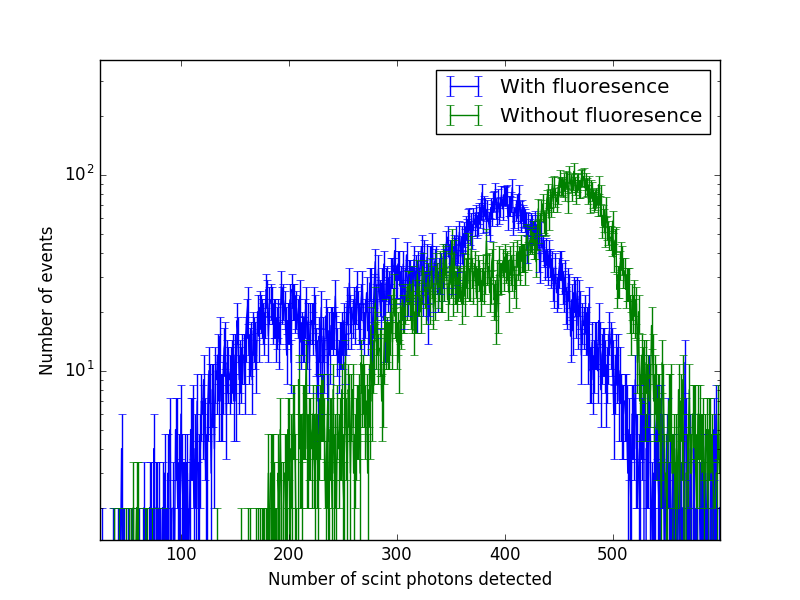
\includegraphics[width=140.0mm]{images/fluovsnofluo.png}
\caption{The obtained energy spectra from simulation with and without x-ray fluoresence being turned on. One can see that, the first peak, which can be seen in the experiments only appear when x-ray fluorescence was turned on.}
\label{fig:fluo}
\end{figure}

\pagebreak

\subsubsection{Calibration of the position dependence}

The main aim of this thesis is to predict what signal the satellite would measure in space. In order to fine tune the parameters of the simulation experimental data was used. The light yield from different parts of the detector is different as scintillation photons have to travel a different distance and they need to be reflected back from the ESR tape that is wrapped around the detector.

\begin{figure}[h!]
\centering
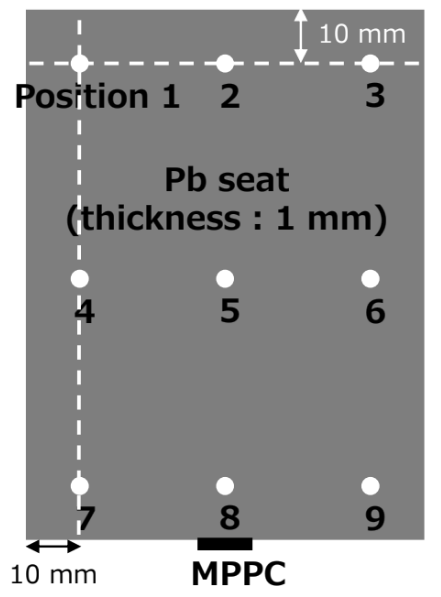
\includegraphics[width=80.0mm]{images/positions.png}
\caption{The positions of irradiation for the investigation of the response of the scintillator  \cite{kento}}
\end{figure}

A lead sheet was drilled with nine holes to collimate the $\gamma$-rays to certain parts of the scintillator. These measurements were carried out by Kento Torigoe at the University of Hiroshima. This configuration with a lead sheet was built up in Geant4 (fig. \ref{fig:this_set} and 3.6 million $\gamma$s were simulated at each position. 

\begin{table}[h!]
\begin{center}
\begin{tabular}{ |c|c|c|c|c|c|c|c|c|c| } 
 \hline
  Pos. of source & 1 & 2 & 3 & 4 & 5 & 6 & 7 & 8 & 9 \\ 
  Pos. of main peak & 0.642 & 0.664 & & 70.7 & 0.743 & & 0.598 & &  \\ 
 \hline
\end{tabular}
\label{tab:exp_sim}
\caption{The position dependence of the photon yield, measured at the Univeristy of Hiroshima by Kento Torigoe}
\end{center}
\end{table}

The three most relevant parameters of the setup in this case are the scintillation photon yield of the scintillator, the reflection rate of the ESR tape and the self-absorption of the scintillator. The photon yield was fixed to 540 $keV^{-1}$ taken from the data sheet of the scintillator \cite{scinti}. The self-absorption and the reflection rate was increased until the position dependence was the same as in the experiment (table. \ref{tabl:simulated}). 

%ADC / energy calibration from measurement 20170829 illetve az egy chanellel: grb\_status3 
\begin{center}

\begin{table}[h!]
\begin{tabular}{ |c|c|c|c|c|c|c|c|c|c| } 
\hline
Refl:& 0.995 & Abs.:& 50 cm   &  &  &  &  &  &  \\ 
\hline
 Pos. of source & 1 & 2 & 3 & 4 & 5 & 6 & 7 & 8 & 9 \\ 
 Pos. of main peak & 0.4013 & 0.3917 & 0.3981 & 0.4045 & 0.4172 & 0.4140 & 0.2580 & 1 & 0.2739\\ 
 \hline   
\hline
 Refl:& 0.997 & Abs.:& 60 cm   &  &  &  &  &  &  \\ 
 \hline
  Pos. of source & 1 & 2 & 3 & 4 & 5 & 6 & 7 & 8 & 9 \\ 
  Pos. of main peak & 0.4588 & 0.4587 & 0.4697 & 0.4734 & 0.4700 & 0.4737 & 0.3388 & 1 & 0.3365  \\ 
 \hline \hline
Refl:& 0.999 & Abs.:& 80 cm   &  &  &  &  &  &  \\ 
 \hline
  Pos. of source & 1 & 2 & 3 & 4 & 5 & 6 & 7 & 8 & 9 \\ 
  Pos. of main peak &  &  &  &  &  &  &  & 1 &   \\ 
 \hline \hline
Refl:& 0.9996 & Abs.:& 80 cm   &  &  &  &  &  &  \\ 
 \hline
  Pos. of source & 1 & 2 & 3 & 4 & 5 & 6 & 7 & 8 & 9 \\ 
  Pos. of main peak &  &  &  &  &  &  &  & 1 &  \\ 
  \hline \hline
Refl:& 0.9999 & Abs.:& 105 cm   &  &  &  &  &  &  \\ 
 \hline
  Pos. of source & 1 & 2 & 3 & 4 & 5 & 6 & 7 & 8 & 9 \\ 
  Pos. of main peak & 0.6911 & 0.6865 & 0.6956 & 0.7002 & 0.6956 & 0.7002 & 0.6041 & 1 & 0.5955 \\ 
  \hline
\end{tabular}
 \caption{The position of the Gaussian peak fitted to the 60 keV peak of the Am source for several irradiated positions. The last set of parameters fit the experimental data.}
 \label{tabl:simulated}
\end{table}
\end{center}

\subsubsection{Calibration of the photon yield}

In the simulation 3.6 million $\gamma$s were simulated. The measurement took 240 s. Therefore the number of photons emitted by the source was $\sim$ 11.0 million. The amplitude of the peaks in the energy spectrum of signal obtained by the MPPC depends mostly on three parameters. The absorption length of the scintillation light in the scintillator, the reflectivity of the surface and the scintillation photon light yield of the scintillator. In order to obtain the histogram that we would measure by the MPPC, the histogram obtained by the simulation had to be scaled up both in amplitude and energy. (The introduction of an offset was not needed as the origin point of the histogram obtained in the measurements was shifted to zero energy.)

\begin{figure}[h!]
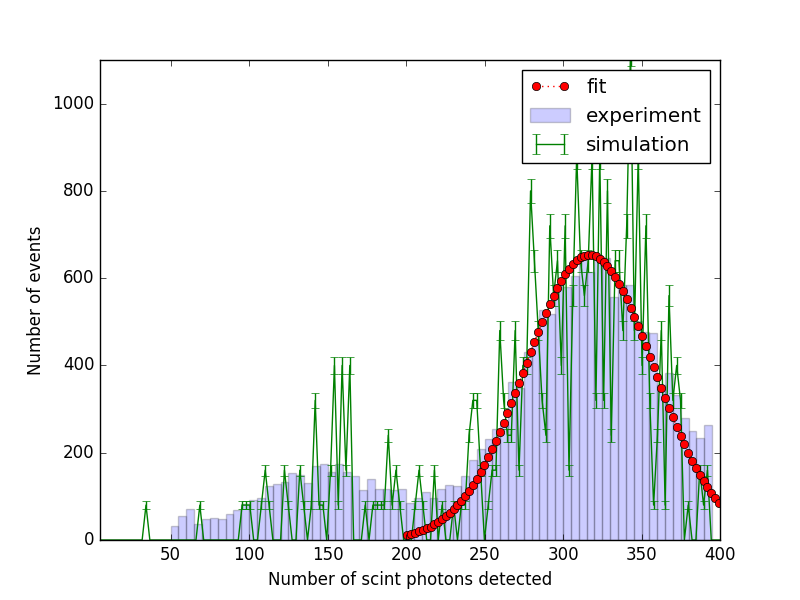
\includegraphics[width=150.0mm]{images/calibration_photon_yield.png}[H!]
\caption{The spectra of 11 million photons taken experimentally \cite{kento} (blue histogram) matched up with the results of the simulation (green histogram) and the Gaussian fitted to the simulated data}
\label{fig:sim_res_calib}
\end{figure}

The energy bins had to be scaled up by a factor of 2.4 to match the experimental results. The amplitude had to be scaled up by a factor of 26.2.

\pagebreak

\subsection{Simulation of the signal induced by GRBs in the satellite} \label{sec:grb}

One of the key questions is what would the satellite measure in space when the $\gamma$ photons of the GRB hit it. It is important to understand how the material of the satellite would absorb the $\gamma$ photons. 

In order to quantify the detection, the number of particles detected was used as a measure. 10,000 $\gamma$ particles were shot at the detector paralelly on an area of 60cm x 60cm from several angles around the longitudinal axis of the satellite. This way the self absorption of the satellite was quantified.

The energy spectra of $\gamma$ photons (called band function) from GRBs is fitted by the following equation \cite{band_func}:

\begin{figure}[h!]
\begin{center}
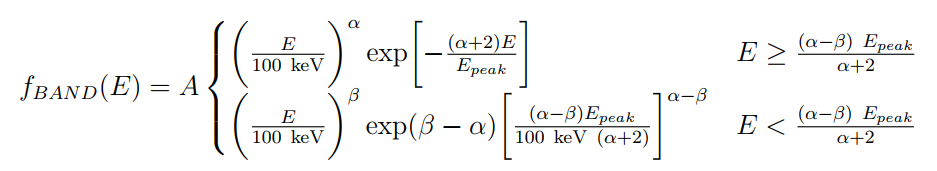
\includegraphics[width=130.0mm]{images/band_function.png}
\label{eq:bandfunc}
\end{center}
\end{figure}

where the parameters of the fit are following for GRB 990123:\\
$\alpha = -0.87 \pm 0.01 $\\
$\beta = -2.9 \pm 0.11$\\
$E_{peak} = (617 \pm 7.09) keV$\\
$A= (0.0262 \pm 0.0000993) s^{-1}cm^{-1}keV^{-1}$\\

Therefore the total flux from GRB 990123 at peak intensity was 9,866 photons for every $cm^{2}$ each second. The illuminated area in the simulation was 3600 cm$^{2}$. Thus the simulated 10,000 photons correspond to 282 $\mu$s. Therefore the number of particles detected in the simulation had to be multiplied by 3551.76 to achive the count number for a second.

\begin{figure}[h!]
\begin{center}
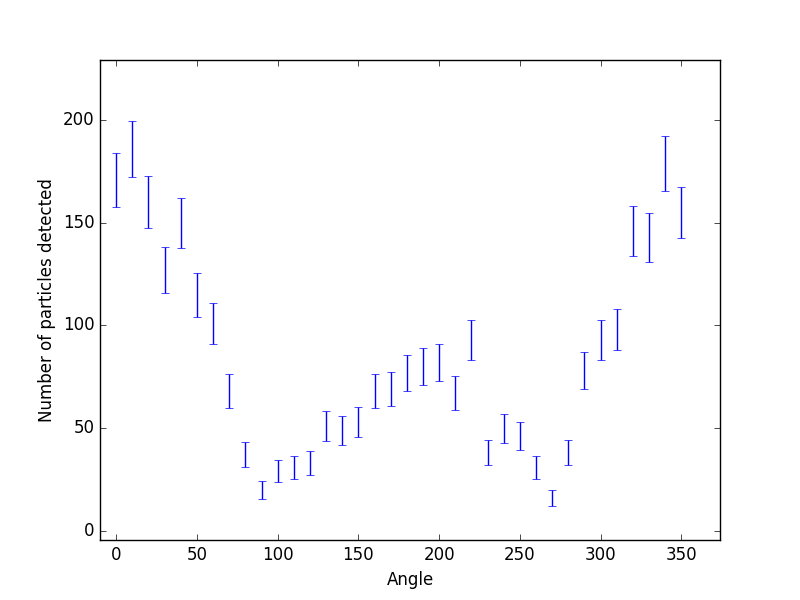
\includegraphics[width=130.0mm]{images/gammashittingsat.png}
\caption{The number of detections from the 10,000 $\gamma$ photons in the simulation depending on the position of the GRB with respect to the longitudinal axis of the satellite.}
\label{fig:diffpos}
\end{center}
\end{figure}

As one expects the most $\gamma$s ($\sim$ 200) are detected when these particles hit the scintillator directly, with a perpendicular direction to the surface of the satellite. The effective area of the scintillator is the largest in this case and the $\gamma$s are not absorbed by the material of the satellite. (Only the aluminium case absorbs $\gamma$-rays in this case.) The detection rate would be 6,393,168 $\frac{Hz}{cm^{2}}$ at peak flux.

The worst case scenario is when the $\gamma$s hit the satellite with a direction parallel to the plane of the scintillator. Although some detections ($\sim$ 20) occur even in this case because $\gamma$s that scatter in the material of the satellite can be detected. In fig. $\ref{fig:diffpos}$ one can see the number of detections from 10,000 $\gamma$s shot at the detector for a given position of the GRB. 

In fig. $\ref{fig:mac17hits}$ one can see the comparison between the energy spectrum measured when the $\gamma$s hit the scintillator in a perpendicular direction and when they hit the satellite from the side opposite to the scintillator. The difference between these two scenarious is that $\gamma$s had to travel through the material of the satellite in the second case. About 60 \% of gammas are lost due to the absorption in the satellite.

\begin{figure}[htbp]
 \centering % \begin{center}/\end{center} takes some additional vertical space
 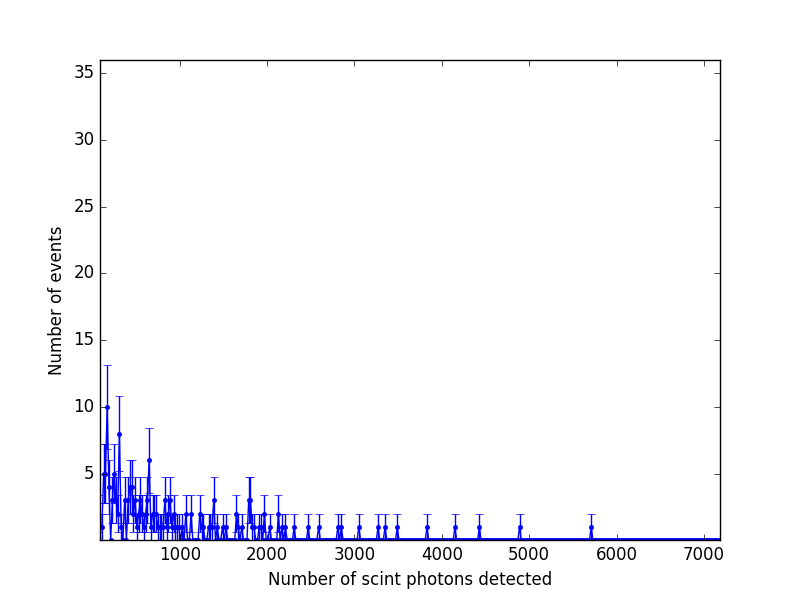
\includegraphics[width=0.45\textwidth,origin=c,angle=0]{images/gamma0mac.png}
 \qquad
 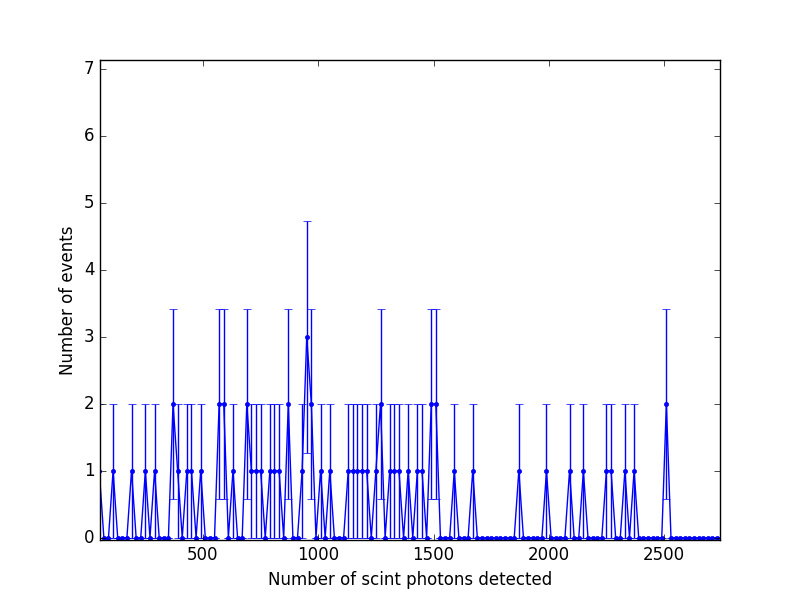
\includegraphics[width=.45\textwidth,origin=c]{images/gamma17mac.png} 
 % "\includegraphics" from the "graphicx" permits to crop (trim+clip)
 % and rotate (angle) and image (and much more)
 \caption{The measured spectrum when the $\gamma$s had to pass through the material of the satellite (right) and when they hit the scintillator directly (left)  \label{fig:mac17hits}}
 \end{figure}


\subsection{Simulation of the cosmic background in space}

In order to understand what would give the measured background of the satellites, cosmic and solar electrons were simulated in the same way as the $\gamma$ particles were in sec. \ref{sec:grb}. The flux of and energy distribution of protons and electrons vary widely in the lower orbits around Earth due to its magnetic field. The SPENVIS \cite{spenvis} information system was used to obtain the proton and electron energy spectra.

SPENVIS is ESA's SPace ENVironment Information System, a WWW interface to models of the space environment and its effects; including cosmic rays, natural radiation belts, solar energetic particles, plasmas, gases, and "micro-particles".

%\subsubsection{Proton background}

%500km\_protons\_max.txt 
%13535.1
%minimum
%12076.5

%In order to include the resonances in the cross section of the hadron-hadron interactions, additional physics models are needed to be included in the simulation. The signal induced by these resonances might affect the measurement of the protons.

%The AE-8 model was used in SPENVIS to obtain the spatially avaraged proton energy spectra for an altitude of 500 km both for solar minimum and maximum. The inclination of the orbit was chosen to be 89 $^{\circ}$. At the moment hadron resonances are not taken into account in the simulation.

%In order to include the resonances in the cross section of the hadron-hadron interactions, additional physics models are needed to be included in the simulation. The signal induced by these resonances might affect the measurement of the protons.

%\begin{figure}[htbp]
% \centering % \begin{center}/\end{center} takes some additional vertical space
% 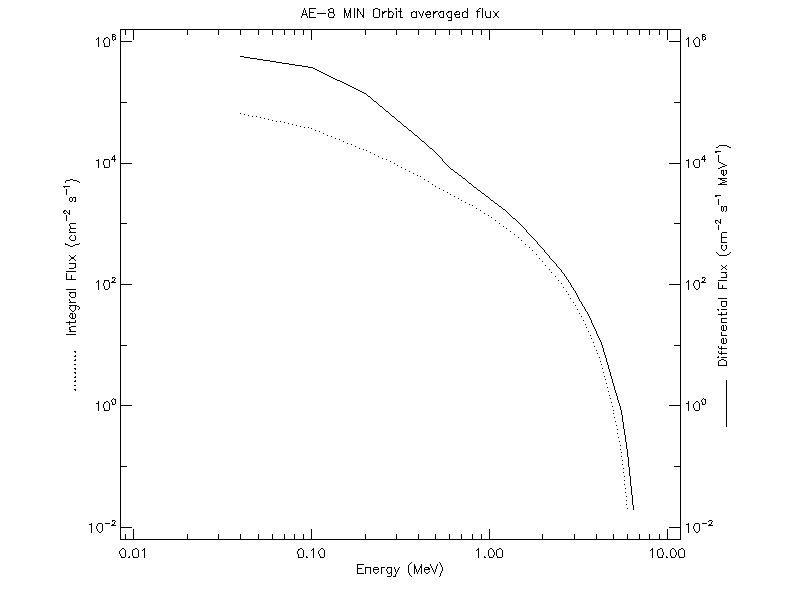
\includegraphics[width=0.45\textwidth,origin=c,angle=0]{images/alt_500km_AE-8_MIN_averaged_spectra.png}
% \qquad
% 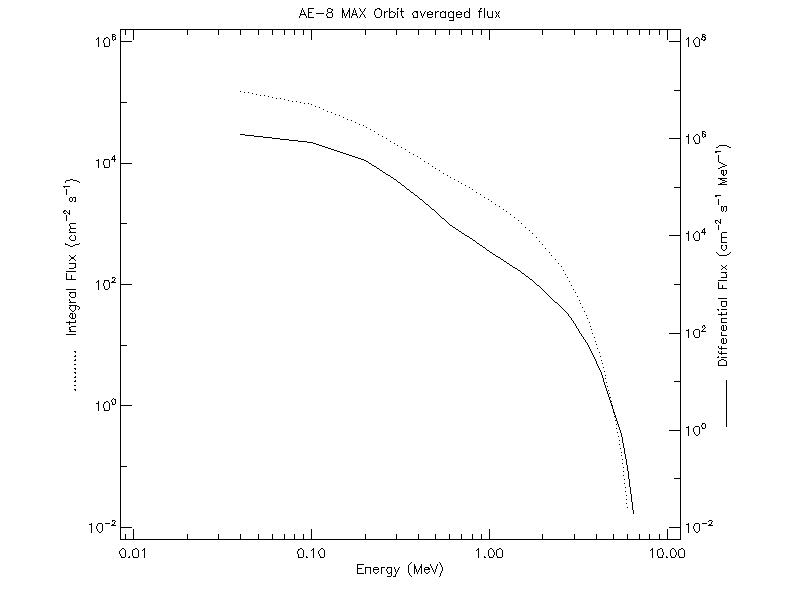
\includegraphics[width=.45\textwidth,origin=c]{images/alt_500km_AE-8_MAX_averaged_spectra.png} 
 % "\includegraphics" from the "graphicx" permits to crop (trim+clip)
 % and rotate (angle) and image (and much more)
% \caption{\label{fig:band500e} The spatially avaraged band function (differential flux for a given energy band, solid line) and the integrated band function (dotted line) of electrons at an altitude of 500 km for solar minimum (left) and solar maximum (right) }
% \end{figure}

%\begin{figure}[htbp]
% \centering % \begin{center}/\end{center} takes some additional vertical space
% 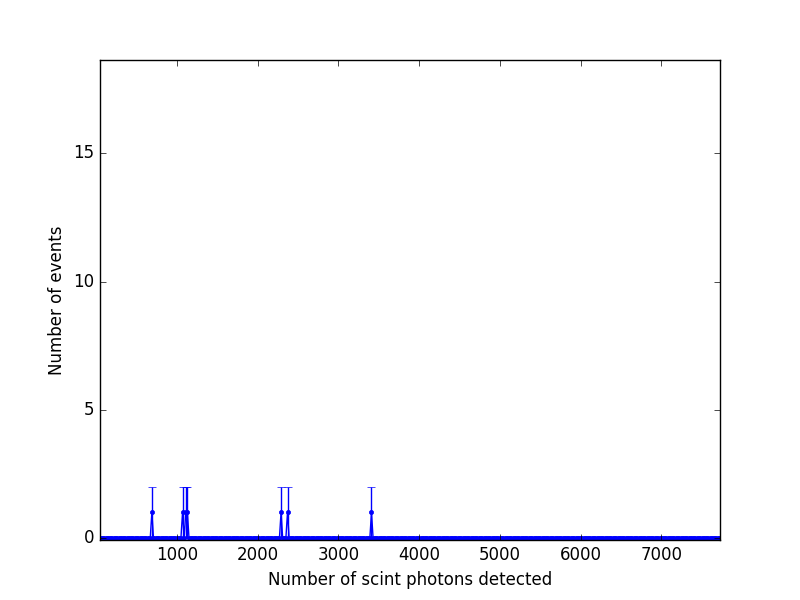
\includegraphics[width=0.45\textwidth,origin=c,angle=0]{images/protons0mac.png}
% \qquad
% 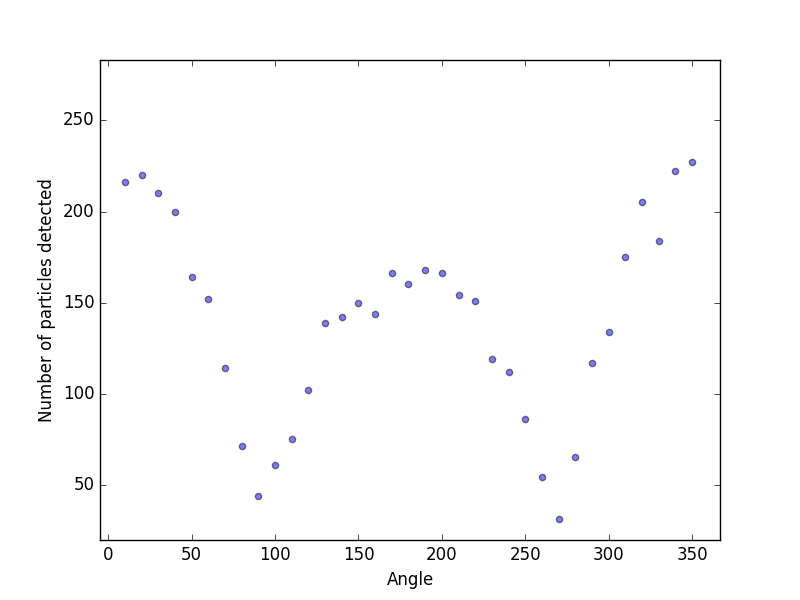
\includegraphics[width=.45\textwidth,origin=c]{images/protonshittingsat.png} 
 % "\includegraphics" from the "graphicx" permits to crop (trim+clip)
 % and rotate (angle) and image (and much more)
 %\caption{\label{fig:band500e}}
 %\end{figure}
%\begin{figure}[h!]
%\begin{center}
%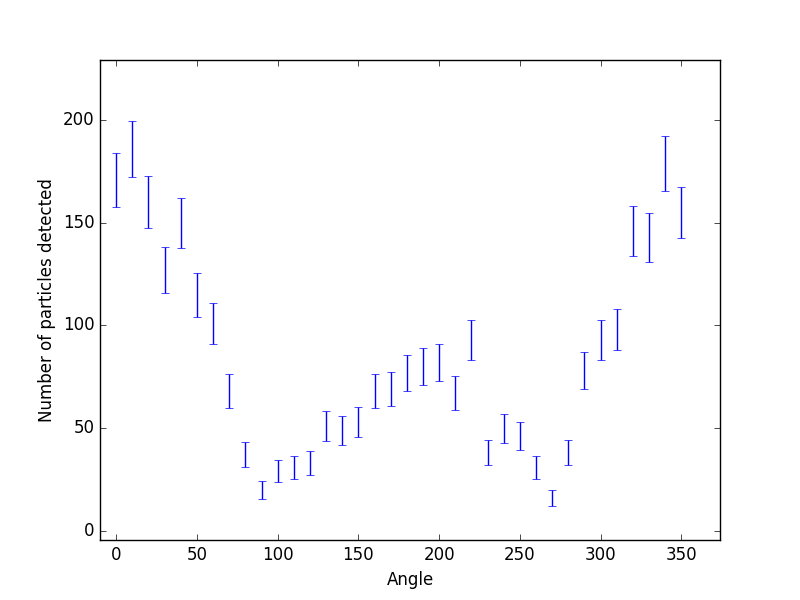
\includegraphics[width=130.0mm]{images/gammashittingsat.png}
%\label{eq:bandfunc}
%\end{center}
%\end{figure}


\subsection{Electron background}

%500km\_electrons\_min.txt
%1.19384e+06
%500km\_electrons  
%2.69537e+06

%'Energy','MeV','Energy'
%'IFlux','cm^-2 s^-1','Integral Flux'
%'DFlux','cm^-2 s^-1 MeV^-1','Differential Flux'

The AE-8 model was used in SPENVIS to obtain the spatially avaraged electron energy spectra for an altitude of 500 km both for solar minimum and maximum. The inclination of the orbit was chosen to be 89$^{\circ}$. %At the moment hadron resonances are not taken into account in the simulation.

\begin{figure}[htbp]
 \centering % \begin{center}/\end{center} takes some additional vertical space
 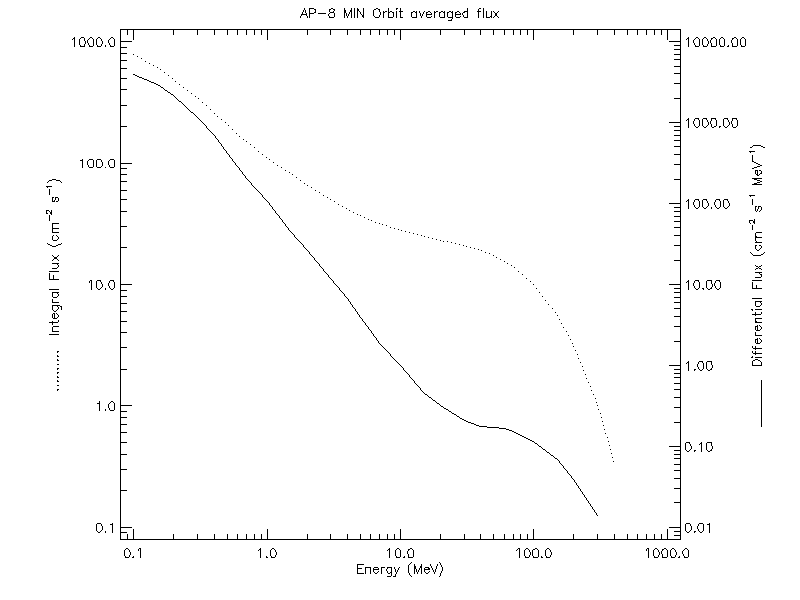
\includegraphics[width=.45\textwidth,origin=c,angle=0]{images/alt_500km_AP-8_MIN_averaged_spectra.png}
 \qquad
 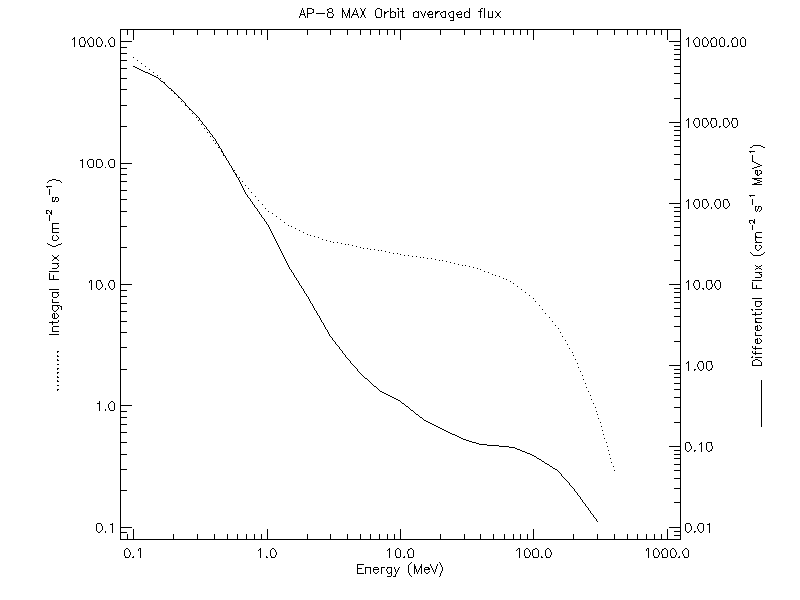
\includegraphics[width=.45\textwidth,origin=c]{images/alt_500km_AP-8_MAX_averaged_spectra.png} 
 % "\includegraphics" from the "graphicx" permits to crop (trim+clip)
 % and rotate (angle) and image (and much more)
 \caption{\label{fig:electrs} The spatially avaraged band function (differential flux for a given energy band, solid line) and the integrated band function (dotted line) of protons at an altitude of 500 km for solar minimum (left) and solar maximum (right) }
 \end{figure}

The integrated and differential spectra of electrons can be seen in fig. \ref{fig:electrs}. For the simulation the worst case scenario, the spectrum at solar maximum was utilized. Fig. \ref{fig:iii} shows the energy spectrum for the simulation of 0$^{\circ}$ when electrons hit the scintillator with a perpendicular direction. 

\begin{figure}[h!]
\centering % \begin{center}/\end{center} takes some additional vertical space
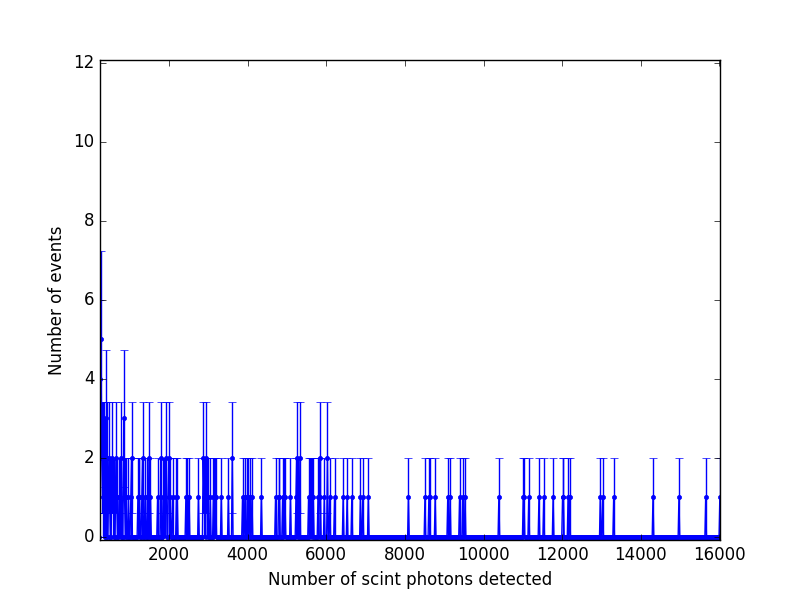
\includegraphics[width=.55\textwidth,origin=c,angle=0]{images/electrons0degspectra.png}
\qquad
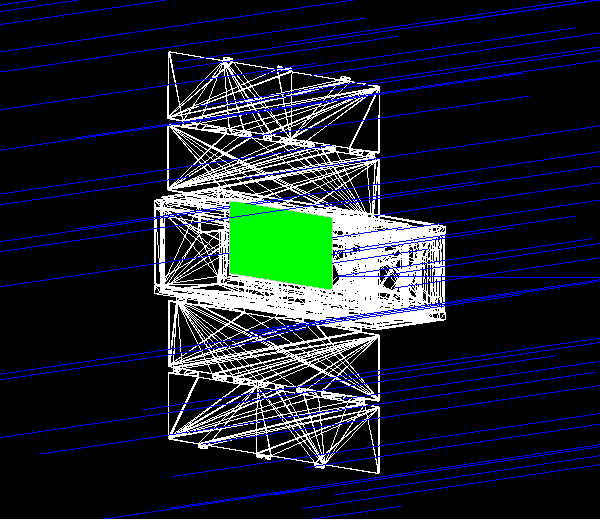
\includegraphics[width=.4\textwidth,origin=c,angle=90]{images/0mac.png} 
% "\includegraphics" from the "graphicx" permits to crop (trim+clip)
% and rotate (angle) and image (and much more)
\caption{\label{fig:iii} The spectrum measured when the electrons were shot perpendicular to the scintillator (called angle of 0 $^{\circ}$)}
\end{figure}

\pagebreak

The total flux from the spectrum taken from SPENVIS (fig. \ref{fig:electrs}) for 1 s and a cm$^{2}$ was 1,226,000. Therefore in order to obtain the count rate, the values obtained for the simulation of 1,000,000 electron with different directions have to be avaraged and multiplied by 1.226 $\cdot$ 3600, which yields 230,478 counts each second.

\begin{figure}[h!]
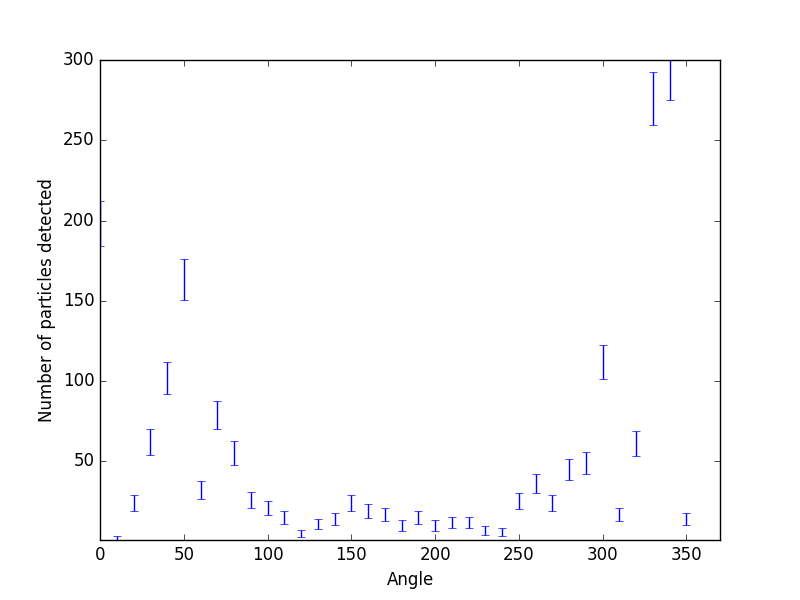
\includegraphics[width=150.0mm]{images/electronabsorption.png}
\caption{The ammount of electrons detected from 1,000,000 shoot in the simulation}
\end{figure}

\pagebreak

\section{Conclusion}

A Geant4 Monte-Carlo based simulation was developed in order to understand how the CAMELOT CubeSat constallation would detect $\gamma$-rays originating from short GRBs. The effect of solar and cosmic electrons on the satellite was also investigated with the simulation.

As the first step, the experimental setup that was used to test the CsI(Tl) scintillator -- the $\gamma$-ray detector of the satellite -- was implemented in Geant4. The optical parameters of the simulation were fine tuned by comparing the light yield of the MPPCs in the simulation with experimental data. After the calibration, the results of the simulation are capable of predicting the signal that would be measured in space.

Secondly, the complex CAD model of the satellite --consisting of 7 modules, each with a given avarage material composition-- was exported to Geant4. The scintillator and its MPPC was placed on the side of the satellite.

Thirdly, the $\gamma$-ray absorption of the satellite was invastigated. Parallel $\gamma$-rays with the energy distribution of the bright GRB 9900123 (fig. \ref{fig:grb_band}) were simulated. 36 positions were investigated by varying the incident angle of the $\gamma$s around the major axis of the satellite.

Fourthly, the effect of cosmic radiation was invastigated by utilizing the energy spectra of cosmic electrons at an altitude of 500km in a polar orbit. It is possible that an other orbit will be choosen for the satellite, as the polar parts of the polar orbit have a very high electron flux.

The satellite was radiated by these particles in Geant4 in the same way that were used for the $\gamma$-rays of GRB 9900123. The induced signal of these particles was determined, which is about one order of magnitude lower than the signal of a GRB. The induced signal of electrons needs to be minimalized as it "competes" with the signal of gamma particles from GRBs.

The results of the simulation shows that the satellite is clearly capable of detecting a GRB with a high signal to noise ratio. The effect of absorption can reduce the measured light yield by 60 \%. The effect of the electron background was also quantified. It is an order of magnitude lower to the signal induced by the $\gamma$-rays of a GRB. 

\pagebreak

\section{Acknowledgment}

G\'abor Galg\'oczi would like to thank Bal\'azs \'Ujv\'ari for the fruitful discussions they had on Geant4 simulations. Useful comments on detectors made Dezs\"o Varga's advices on detectors were highly appreciated. The model of the satellite was provided by Norbert Tarcai and Olivér Wágner from C3S LLC. The experimental data that was needed for the simulation was provided by Kento Torigoe and his colleges from the University of Hiroshima. The energy spectrum of cosmic electrons was deduced by Jakub Ripa. Last but not least the author would like to thank Norbert Werner for the continued contributions to this work.  

\pagebreak

\addcontentsline{toc}{section}{References}
\begin{thebibliography}{99}
\interlinepenalty=10000

\bibitem{grb1} Mészáros P., 2006, Reports on Progress in Physics, 69, 2259
%https://link.springer.com/content/pdf/10.1007/s11214-017-0366-4.pdf

\bibitem{grb2} Vedrenne G., \& Atteia J.-L., 2009, Gamma-Ray Bursts: The brightest explosions in the Universe,
Springer Praxis Books in Astronomy and Planetary Sciences, Published in association with Praxis
Publishing, UK
%https://link.springer.com/content/pdf/10.1007/s11214-017-0366-4.pdf

\bibitem{grb3} Kouveliotou C., Wijers R. A. M. J., \& Woosley S., 2012, Gamma-ray Bursts, Cambridge, UK:
Cambridge University Press
%https://link.springer.com/content/pdf/10.1007/s11214-017-0366-4.pdf

\bibitem{grb4} Gehrels N., \& Mészáros P. 2012, Science, 337, 932
%https://link.springer.com/content/pdf/10.1007/s11214-017-0366-4.pdf

\bibitem{grb5} Klebesadel R. W., Strong I. B., \& Olson R. A. 1973, The Astrophysical Journal, 182, L85

\bibitem{grb6} Kouveliotou C., Meegan C. A., Fishman G. J., et al. 1993, The Astrophysical Journal Letters, 413, L101

\bibitem{grb7} Balázs L. G., Bagoly Z., Horváth I., et al. 2003, Astronomy and Astrophysics, 401, 129

\bibitem{grb8} Mészáros A., Bagoly Z., Balázs L. G., \& Horváth I. 2006, Astronomy and Astrophysics, 455, 785

\bibitem{grb9} Berger E. 2014, Annual Review of Astronomy and Astrophysics, 52, 43

\bibitem{grb10} Rees M. J., \& Meszaros P. 1994, The Astrophysical Journal, 430, L93

\bibitem{grb11} van Paradijs J., Groot P. J., Galama T., et al. 1997, Nature, 386, 686

\bibitem{grb12} Paczynski B. 1986, The Astrophysical Journal, 308, L43

\bibitem{grb14} Fruchter A. S., Levan A. J., Strolger L., et al. 2006, Nature, 441, 463

\bibitem{gravwave} https://arxiv.org/abs/1710.05834

\bibitem{grb17} Abbott B. P., Abbott R., Abbott T. D., et al. 2017, Physical Review Letters, 119, 161101

\bibitem{grb18} Tanvir N. R., Levan A. J., Fruchter A. S., et al. 2013, Nature, 500, 547

\bibitem{grb19} Zhang, B. 2011, Comptes Rendus Physique, 12, 206

\bibitem{grb20} Toma, K., Yoon, S.-C., \& Bromm, V. 2016, Space Science Reviews, 202, 159

\bibitem{grb21} Goldstein A., et al., 2017, The Astrophysical Journal Letters, 848, L14

\bibitem{grb22} Savchenko V., et al., 2017, The Astrophysical Journal Letters, 848, L15

\bibitem{grb23} Troja E., et al., 2017, Naure, 551, 71

\bibitem{grb24} Evans P. A., Cenko S. B., Kennea J. A., et al. 2017, Science, 358, 1565

\bibitem{grb25} Loeb A., 2016, The Astrophysical Journal Letters, 819, L21

\bibitem{grb26} KAGRA Collaboration, Akutsu T., Ando M., et al. 2017, arXiv:1710.04823

\bibitem{grb27} Cavallari E., \& Frontera F. 2017, Space Science Reviews, 212, 429
 
\bibitem{grb28} Atwood, W. B., \& GLAST Collaboration 1994, Nuclear Instruments and Methods in Physics Research
A, 342, 302

\bibitem{grb30} Cavallari E., \& Frontera F. 2017, Space Science Reviews, 212, 429

\bibitem{grb31} Barthelmy S. D., Barbier L. M., Cummings J. R., et al. 2005, Space Science Reviews, 120, 143

\bibitem{grb32} Winkler C., Courvoisier T. J.-L., Di Cocco G., et al. 2003, Astronomy and Astrophysics, 411, L1

\bibitem{grb34} Tavani M., Barbiellini G., Argan A., et al. 2009, Astronomy and Astrophysics, 502, 995

\bibitem{grb35} Yamaoka K., Yoshida A., Nonaka Y. 2011, 32nd International Cosmic Ray Conference, 9, 111

\bibitem{grb36} Serino M., Sakamoto T., Kawai N., et al. 2014, Publications of the Astronomical Society of Japan, 66,
87

\bibitem{grb37} Produit N., Barao F., Deluit S., et al. 2005, Nuclear Instruments and Methods in Physics Research A,
550, 616

\bibitem{grb38} Sadovnichii V. A., Panasyuk M. I., Amelyushkin A. M., et al. 2017, Space Science Reviews, 212, 1705

\bibitem{grb39} Li T., Xiong S., Zhang S., et al. 2018, Science China Physics, Mechanics, and Astronomy, 61, 31011

\bibitem{grb40} Navalgund K. H., Suryanarayana Sarma K., Gaurav P. K., Nagesh G., \& Annadurai M. 2017, Journal of Astrophysics and Astronomy, 38, 34

\bibitem{grb41} Lin R. P., Dennis B. R., Hurford G. J., et al. 2002, Solar Physics, 210, 3

\bibitem{drawing} Private communication, C3S LLC.

\bibitem{kento} Master thesis, K. Torigoe, N. Werner, Y. Fukazawa, N. Uchida, K. Tanaka, T. Mizuno \& H. Takahashi, School of Science, Hiroshima University,

%\bibitem{kento} Master thesis, K. Torigoe, Norbert Werner, Yasushi Fukazawa, Nagomi Uchida, Koji Tanaka, Tsunefumi Mizuno \& Hiromitsu Takahashi, School of Science, Hiroshima University,

\bibitem{grb42} Hurley K., Mitrofanov I. G., Golovin D., et al. 2013, EAS Publications Series, 61, 459 

\bibitem{grb43} Lipunov V., Kornilov V., Gorbovskoy E., et al. 2016, Revista Mexicana de Astronomia y Astrofisica
Conference Series, 48, 42

\bibitem{grb44} Castro-Tirado A. J., Soldán J., Bernas M., et al. 1999, Astronomy and Astrophysics Supplement, 138, 583

\bibitem{grb45} Akerlof C. W., Kehoe R. L., McKay T. A., et al. 2003, Publications of the Astronomical Society of the Pacific, 115, 132

\bibitem{grb46} Majcher A., Batsch T., Castro-Tirado A. J., et al. 2015, Proceedings of SPIE, 9662, 966219

\bibitem{grb_spectra} Gamma-Ray Bursts and Fast Transients
Multi-wavelength Observations and Multi-messenger Signals,\\
R. Willingale, P. Mészáros
%https://link.springer.com/content/pdf/10.1007/s11214-017-0366-4.pdf

\bibitem{geant1} Nuclear Instruments and Methods in Physics Research A 506 (2003) 250-303

\bibitem{geant2} IEEE Transactions on Nuclear Science 53 No. 1 (2006) 270-278

\bibitem{geant3} Nuclear Instruments and Methods in Physics Research A 835 (2016) 186-225

\bibitem{cadmesh} Poole, C. M. and Cornelius, I. and Trapp, J. V. and Langton, C. M., A CAD Interface for GEANT4, Australasian Physical \& Engineering Science in Medicine, 2012

\bibitem{assimp} http://www.assimp.org/

\bibitem{tetgen} Hang Si. 2015. "TetGen, a Delaunay-Based Quality Tetrahedral Mesh Generator". ACM Trans. on Mathematical Software. 41 (2), Article 11 (February 2015), 36 pages

\bibitem{scinti} http://www.amcrys.com/pdf/4279\_.pdf

\bibitem{qe} http://www.hamamatsu.com/resources/pdf/ssd/s13360\_series\_kapd1052e.pdf

\bibitem{esr} http://multimedia.3m.com/mws/media/466120O/esr.pdf
 
\bibitem{band_func} https://arxiv.org/pdf/1311.7135.pdf
 
 
\bibitem{spenvis} https://www.spenvis.oma.be/

\end{thebibliography}

\pagebreak

\listoffigures

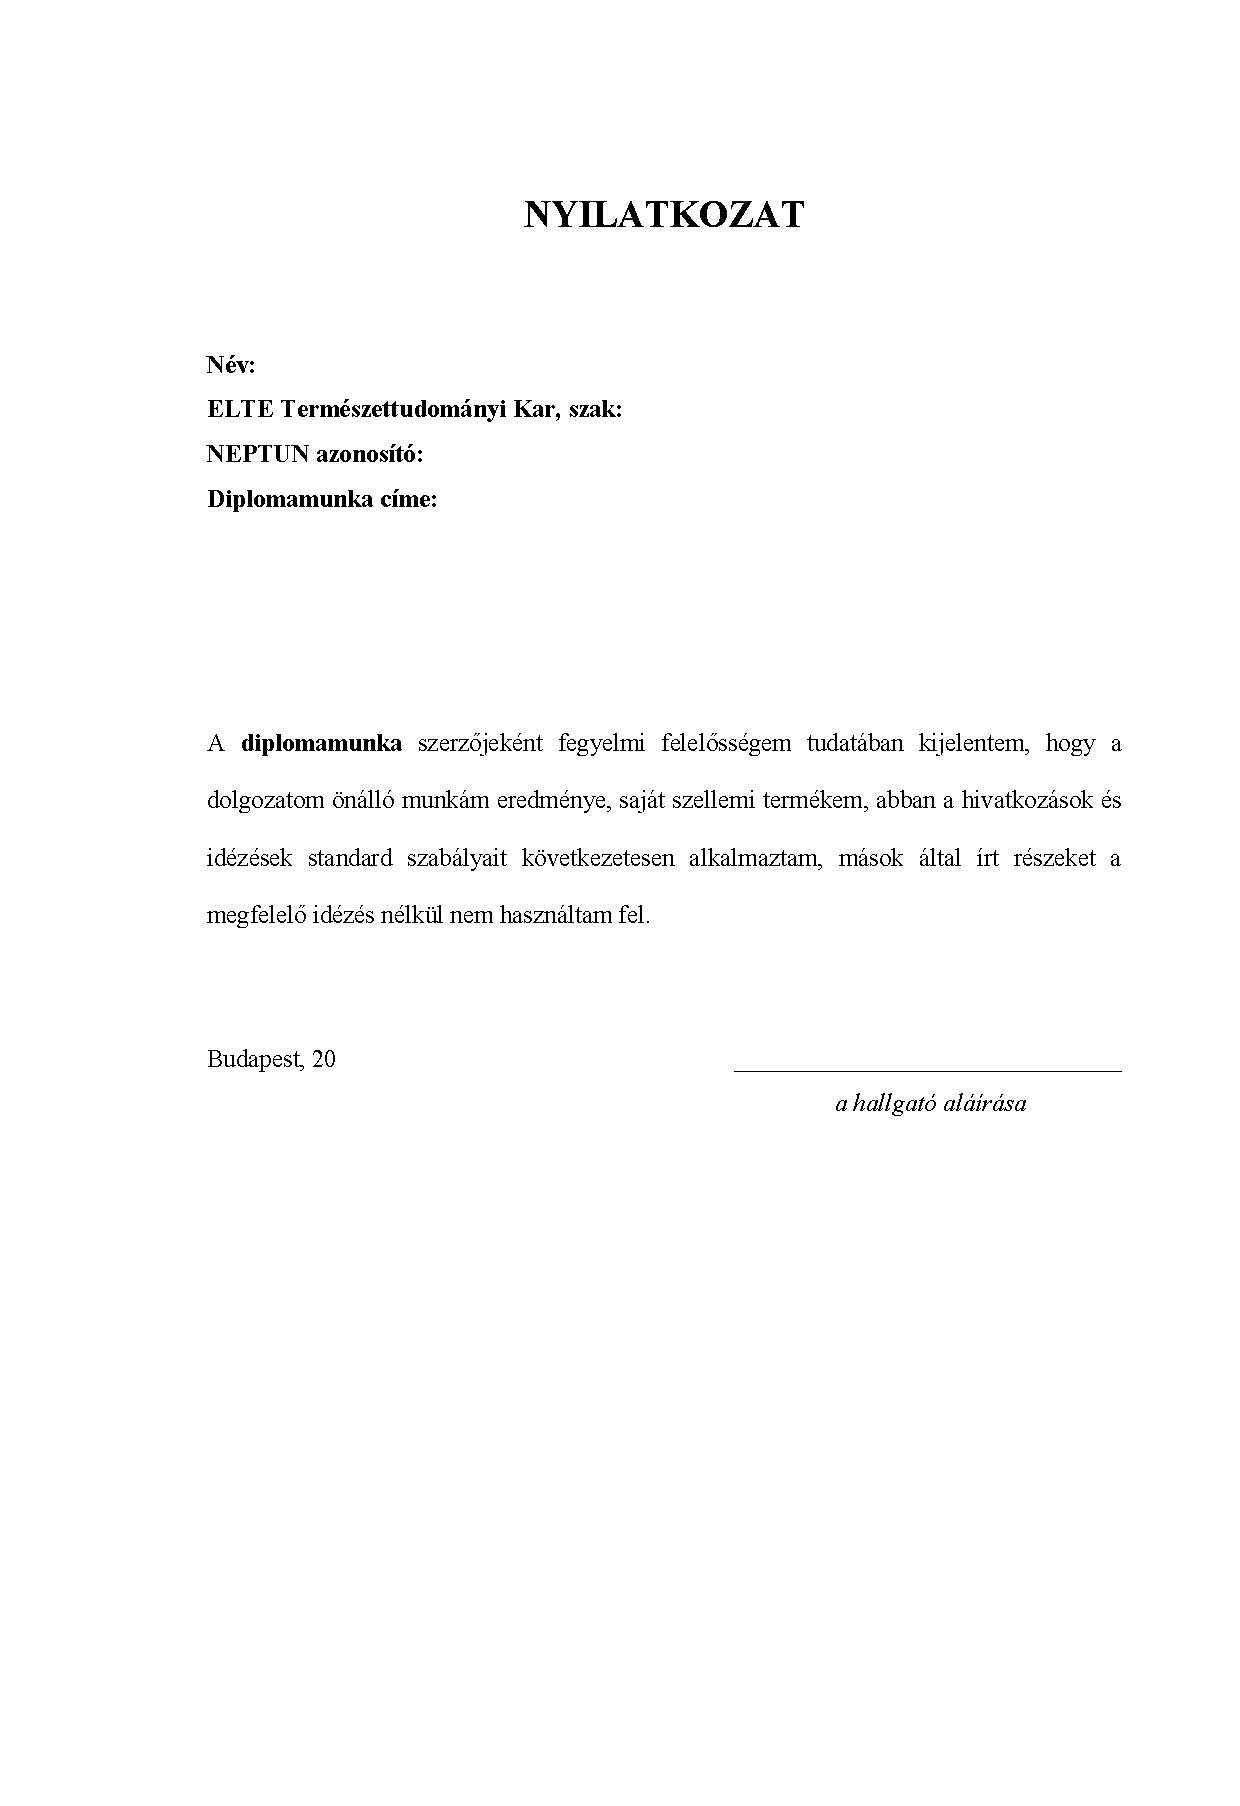
\includepdf[pages=-,pagecommand={},width=\textwidth]{images/nyilatkozat.pdf}



\end{document}

\begin{figure}[h!]
\centerline{
\includegraphics[width=260pt,angle=0]{images/let_setup.png}}
\caption{Az általam használt OTPC a gázrendszerével, illetve a kiolvasórendszerével együtt}
\end{figure}

Sötét anyag kutatásra jó beveztő:
https://arxiv.org/pdf/1510.02170.pdf
Nuclear physics:
https://indico.fnal.gov/conferenceDisplay.py/abstractBook?confId=8976

%%%%%%%%%%%%%%%
Alkalmazások


M. Pomorski, M. Pfutzner
M. Pomorski et al. Phys. Rev. C 90, 014311 (2014)

Micromegas-os kiolvasás J. B. R. Battat, Nucl. Instr. Meth. A 755(2014)6.

[grid???] U. Titt, V. Dagendorf et al., (Nucl. Instr. Meth. A 477 (2002) 536:	 
grids, pure TEA at low pressure, (electron counting / nano-dosimetry)

%%%%%%%%%%%%%%

Performance of an optical readout GEM-based TPC, L.M.S. Margato a...

optikai úton kiolvasott tpc-k: florian e-mailjéből

LET TPC

radon és polónium energiáira cikkek